% filepath: /home/hrishikesh/Desktop/AI_semII/lab_report_cycle_II.tex
\documentclass[a4paper,12pt]{article}
\usepackage{fancyhdr}
\usepackage{geometry}
\usepackage{lipsum}
\usepackage{longtable}
\usepackage{titlesec}
\usepackage{hyperref}
\usepackage{listings}
\usepackage{etoolbox}
\usepackage{graphicx}
\usepackage{amsmath}

% Page geometry and shifting
\geometry{left=2.5cm,right=2.5cm,top=2.5cm,bottom=2.5cm}
\newcommand{\oddshift}{\hspace*{-1cm}}
\newcommand{\evenshift}{\hspace*{1cm}}

% Fancyhdr for footer
\setlength{\footskip}{30pt}
\pagestyle{fancy}
\fancyhf{}  % clear all headers and footers
\renewcommand{\headrulewidth}{0pt}

\fancyfoot[C]{
  \begin{minipage}{\textwidth}
    \centering
    \rule{\textwidth}{1.5pt}\\
    Pattern Recognition Laboratory
  \end{minipage}
}
\fancyfoot[R]{\thepage}

% Shift content on odd/even pages
\makeatletter
\patchcmd{\@outputpage@head}{\box\@outputbox}{%
  \ifodd\value{page}\oddshift\else\evenshift\fi\box\@outputbox
}{}{}
\makeatother

% Section formatting
\titleformat{\section}
  {\normalfont\Large\bfseries\centering}{\thesection}{1em}{}
\titleformat{\subsection}
  {\normalfont\large\bfseries}{\thesubsection}{1em}{}

% Listings for code
\lstset{
  basicstyle=\ttfamily\small,
  frame=single,
  breaklines=true,
  showstringspaces=false
}

\begin{document}


% Index/Table of Contents
\section*{Index}
\begin{longtable}{|c|p{9cm}|c|}
\hline
\textbf{Sl No} & \textbf{Name of the program} & \textbf{Page No} \\
\hline
1 & [Program Name 1] & \pageref{exp1} \\
2 & [Program Name 2] & \pageref{exp2} \\
3 & [Program Name 3] & \pageref{exp3} \\
% ... Add more as needed ...
\hline
\end{longtable}
\newpage

% --- Experiment 1 Example ---
\section*{Cycle II}
\begin{center}
\textbf{Experiment 1}
\label{exp1}
\end{center}

\vspace{1em}

\raggedright{
  \textbf{Problem}\par
  \noindent
  Apply LDA for dimensionality reduction and any classifier for face recognition on the ORL dataset and analyze the performance.\par
}


\vspace{1em}

\textbf{Aim and Objectives}

To implement LDA for dimensionality reduction and evaluate its effectiveness in improving the performance of a face recognition classifier on the ORL dataset.

\vspace{1em}

\textbf{Program Code}

\begin{lstlisting}[language=Python]
import os
import cv2
import matplotlib.pyplot as plt
import shutil
import pandas as pd
import numpy as np
import seaborn as sns
from sklearn.model_selection import train_test_split
from sklearn.discriminant_analysis import LinearDiscriminantAnalysis as LDA
from sklearn.metrics import accuracy_score, confusion_matrix, classification_report
from sklearn.svm import SVC


dataset_path = "../datasets/ORL_dataset"

\end{lstlisting}

\begin{lstlisting}[language=Python]
classes = os.listdir(dataset_path)

\end{lstlisting}

\begin{lstlisting}[language=Python]
plt.subplots(5, 8, figsize=(15, 12.5))
plt.suptitle("Sample Images from ORL Dataset", fontsize=12)
for class_name in classes:
    image = cv2.imread(os.path.join(dataset_path, class_name, "1.pgm"), cv2.IMREAD_GRAYSCALE)
    plt.subplot(5, 8, classes.index(class_name) + 1)
    plt.imshow(image, cmap='gray')
    plt.title(f"{class_name}")

\end{lstlisting}

\begin{center}
  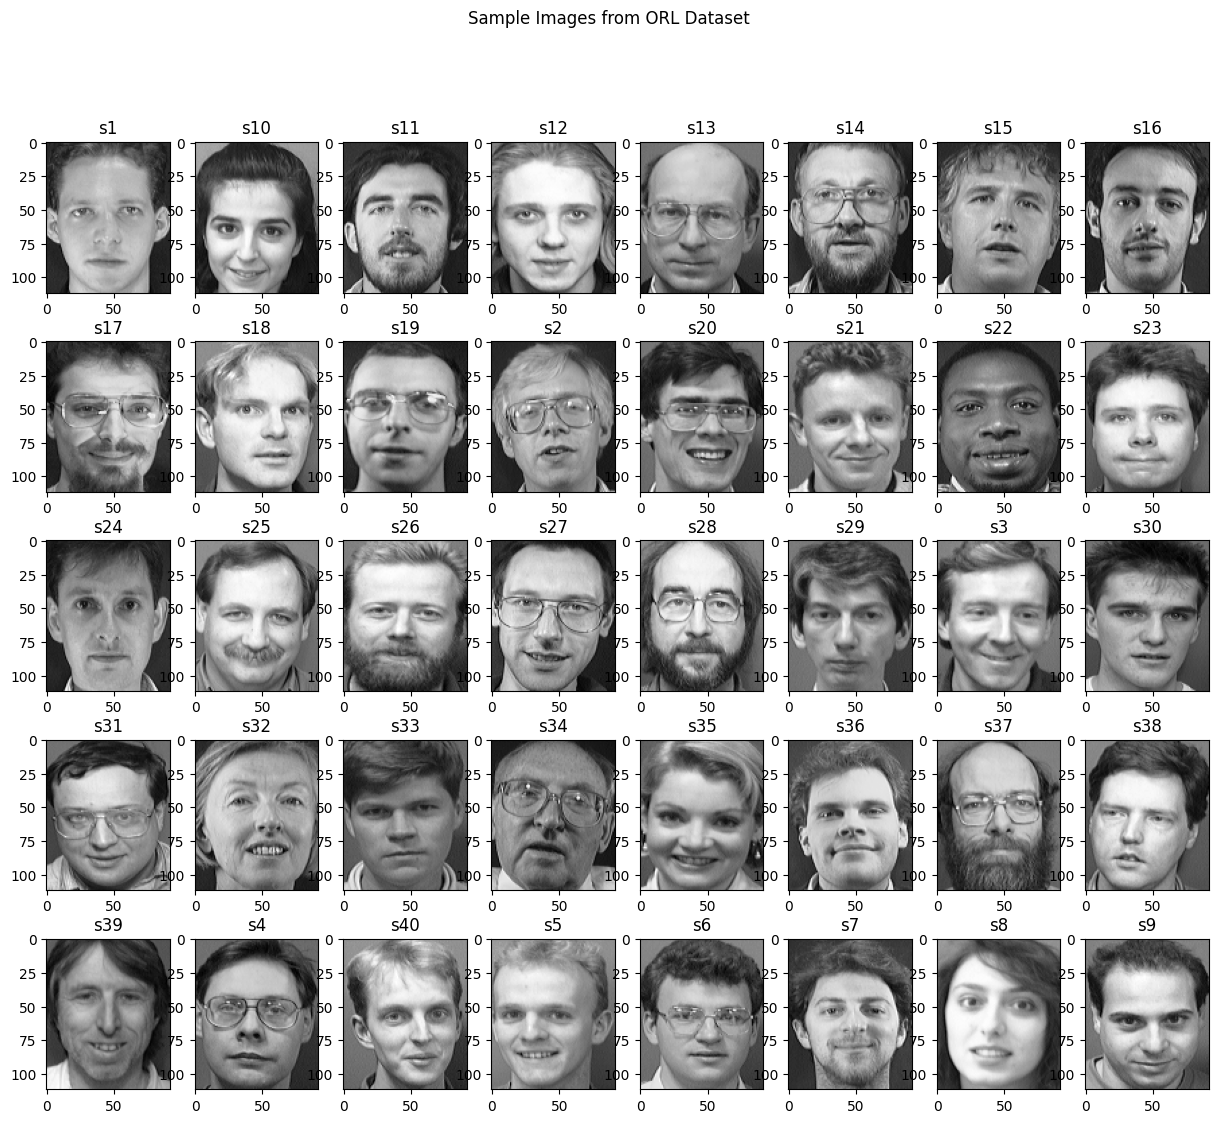
\includegraphics[width=0.8\textwidth]{output_01.png}
\end{center}


\begin{lstlisting}[language=Python]
test_ratio = 0.2

classes = os.listdir(dataset_path)

for class_name in classes:

    os.makedirs(f"../datasets/train/{class_name}", exist_ok=True)
    os.makedirs(f"../datasets/test/{class_name}", exist_ok=True)

    images = os.listdir(f"../datasets/ORL_dataset/{class_name}")
    train_images, test_images = train_test_split(images, test_size=test_ratio, random_state=42)

    for img in train_images:
        shutil.copy(f"../datasets/ORL_dataset/{class_name}/{img}", f"../datasets/train/{class_name}/{img}")
    print(f"Copied images for {class_name} to train folder")

    for img in test_images: 
        shutil.copy(f"../datasets/ORL_dataset/{class_name}/{img}", f"../datasets/test/{class_name}/{img}")
    print(f"Copied images for {class_name} to test folder")


\end{lstlisting}

\vspace{\baselineskip}
\vspace{\baselineskip}

\begin{lstlisting}[language=Python]
train_set = "../datasets/train"
test_set = "../datasets/test"
\end{lstlisting}

\begin{lstlisting}[language=Python]
images_X = []
labels_y = []
for class_name in classes:
    class_path = os.path.join(train_set, class_name)
    for img_name in os.listdir(class_path):
        img_path = os.path.join(class_path, img_name)
        image = cv2.imread(img_path, cv2.IMREAD_GRAYSCALE)
        images_X.append(image.flatten())
        labels_y.append(classes.index(class_name))
print(f"Number of images in train set: {len(images_X)}")
\end{lstlisting}

\begin{lstlisting}[language=Python]
  Number of images in train set: 320
\end{lstlisting}

\begin{lstlisting}[language=Python]
labels_y = np.array(labels_y)
images_X = pd.DataFrame(images_X)
\end{lstlisting}

\begin{lstlisting}[language=Python]
lda = LDA(n_components=39)
images_X_lda = lda.fit_transform(images_X, labels_y)
images_X_lda_df = pd.DataFrame(images_X_lda)
images_X_lda_df
\end{lstlisting}

\begin{center}
  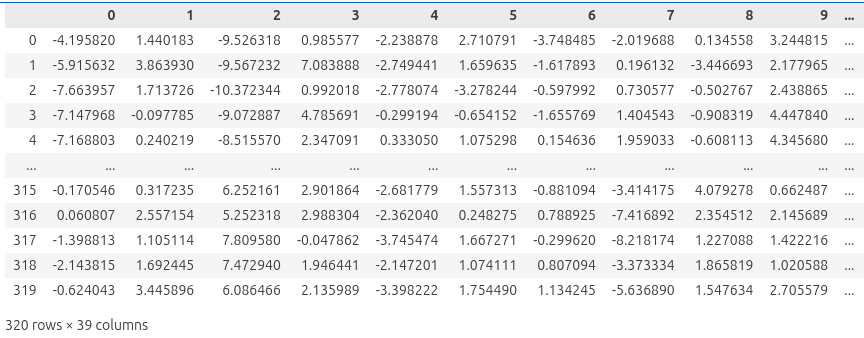
\includegraphics[width=0.8\textwidth]{output_02.png}
\end{center}

\begin{lstlisting}[language=Python]
test_images_X = []
test_labels_y = []
for class_name in classes:
    class_path = os.path.join(test_set, class_name)
    for img_name in os.listdir(class_path):
        img_path = os.path.join(class_path, img_name)
        image = cv2.imread(img_path, cv2.IMREAD_GRAYSCALE)
        test_images_X.append(image.flatten())
        test_labels_y.append(classes.index(class_name))
\end{lstlisting}

\begin{lstlisting}[language=Python]
test_images_X_df = pd.DataFrame(test_images_X)
test_labels_y = np.array(test_labels_y)
\end{lstlisting}

\begin{lstlisting}[language=Python]
test_images_X_lda = lda.transform(test_images_X_df)
test_images_X_lda_df = pd.DataFrame(test_images_X_lda)
\end{lstlisting}

\begin{lstlisting}[language=Python]
Training SVM with LDA applied on the features
\end{lstlisting}

\begin{lstlisting}[language=Python]
svm_01 = SVC(kernel="linear", gamma="scale")
svm_01.fit(images_X_lda, labels_y)
\end{lstlisting}

\begin{center}
  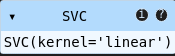
\includegraphics[width=0.25\textwidth]{output_03.png}
\end{center}

\begin{lstlisting}[language=Python]
y_pred = svm_01.predict(test_images_X_lda)
cl_report = classification_report(test_labels_y, y_pred, target_names=classes)
print(cl_report)
\end{lstlisting}

\begin{lstlisting}[language=Python]
              precision    recall  f1-score   support

          s1       1.00      0.50      0.67         2
         s10       1.00      1.00      1.00         2
         s11       1.00      1.00      1.00         2
         s12       1.00      1.00      1.00         2
         s13       1.00      1.00      1.00         2
         s14       1.00      1.00      1.00         2
         s15       1.00      1.00      1.00         2
         s16       0.67      1.00      0.80         2
         s17       1.00      1.00      1.00         2
         s18       1.00      1.00      1.00         2
         s19       1.00      1.00      1.00         2
          s2       1.00      1.00      1.00         2
         s20       1.00      1.00      1.00         2
         s21       1.00      1.00      1.00         2
         s22       1.00      1.00      1.00         2
         ...

    accuracy                           0.96        80
   macro avg       0.97      0.96      0.96        80
weighted avg       0.97      0.96      0.96        80
\end{lstlisting}

\begin{lstlisting}[language=Python]
ac_score = accuracy_score(test_labels_y, y_pred)
print(f"Accuracy of the SVM model on test set: {ac_score}")
\end{lstlisting}

\begin{lstlisting}[language=Python]
Accuracy of the SVM model on test set: 0.9625
\end{lstlisting}

\begin{lstlisting}[language=Python]
cf = confusion_matrix(test_labels_y, y_pred)
plt.figure(figsize=(12, 10))
sns.heatmap(cf, annot=True, fmt='d', cmap='Blues', xticklabels=classes, yticklabels=classes)
plt.title("Confusion Matrix for SVM Model")
\end{lstlisting}

\begin{center}
  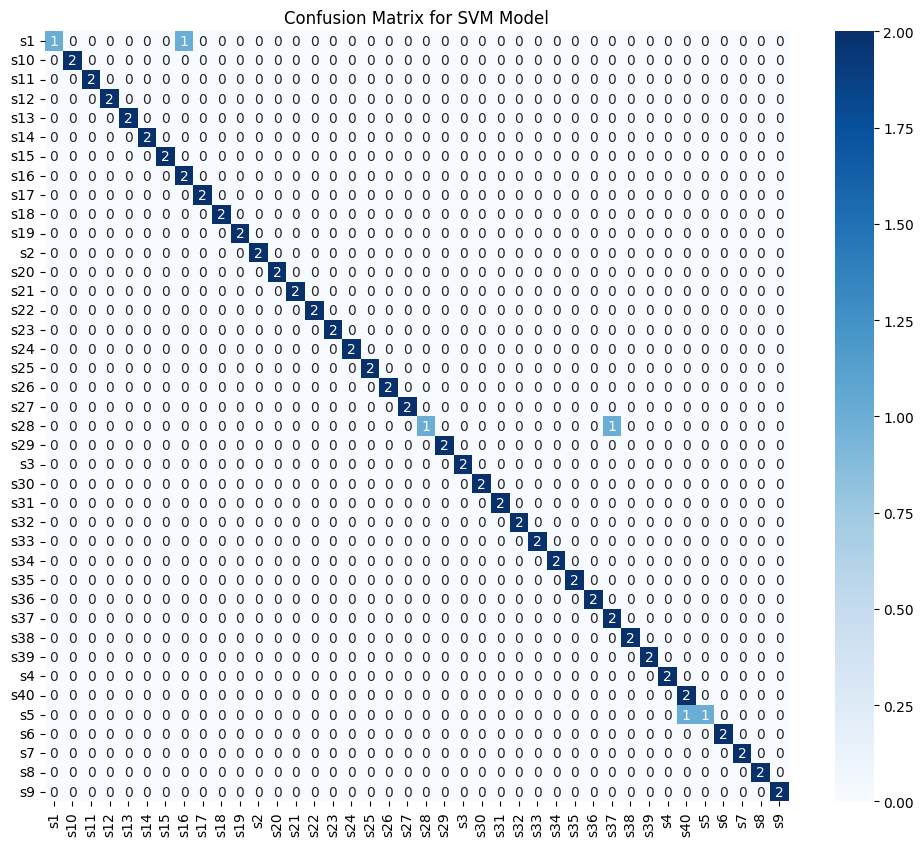
\includegraphics[width=0.8\textwidth]{output_04.png}
\end{center}

\begin{lstlisting}[language=Python]
Training SVM with original features
\end{lstlisting}

\begin{lstlisting}[language=Python]
svm_02 = SVC(kernel="linear", gamma="scale")
svm_02.fit(images_X, labels_y)
\end{lstlisting}

\begin{lstlisting}[language=Python]
y_pred_02 = svm_02.predict(test_images_X_df)
cl_report_02 = classification_report(test_labels_y, y_pred_02, target_names=classes)
print(cl_report_02)
\end{lstlisting}

\begin{lstlisting}[language=Python]
              precision    recall  f1-score   support

          s1       1.00      1.00      1.00         2
         s10       1.00      0.50      0.67         2
         s11       1.00      1.00      1.00         2
         s12       1.00      1.00      1.00         2
         s13       1.00      1.00      1.00         2
         s14       1.00      1.00      1.00         2
         s15       1.00      1.00      1.00         2
         s16       1.00      1.00      1.00         2
         s17       1.00      1.00      1.00         2
         s18       0.67      1.00      0.80         2
         s19       1.00      1.00      1.00         2
          s2       1.00      1.00      1.00         2
         s20       1.00      1.00      1.00         2
         s21       1.00      1.00      1.00         2
         s22       1.00      1.00      1.00         2
         s23       1.00      1.00      1.00         2
         s24       1.00      1.00      1.00         2
         s25       1.00      1.00      1.00         2
         s26       1.00      1.00      1.00         2
         s27       1.00      1.00      1.00         2
         s28       1.00      0.50      0.67         2
         s29       1.00      1.00      1.00         2
          s3       1.00      1.00      1.00         2
...
    accuracy                           0.96        80
   macro avg       0.97      0.96      0.96        80
weighted avg       0.97      0.96      0.96        80
\end{lstlisting}

\begin{lstlisting}[language=Python]
ac_score_02 = accuracy_score(test_labels_y, y_pred_02)
print(f"Accuracy of the SVM model on test set without LDA: {ac_score_02}")
\end{lstlisting}

\begin{lstlisting}[language=Python]
Accuracy of the SVM model on test set without LDA: 0.9625
\end{lstlisting}

\begin{lstlisting}[language=Python]
cf_02 = confusion_matrix(test_labels_y, y_pred_02)
plt.figure(figsize=(12, 10))
sns.heatmap(cf_02, annot=True, fmt='d', cmap='Blues', xticklabels=classes, yticklabels=classes)
plt.title("Confusion Matrix for SVM Model without LDA")
\end{lstlisting}

\begin{center}
  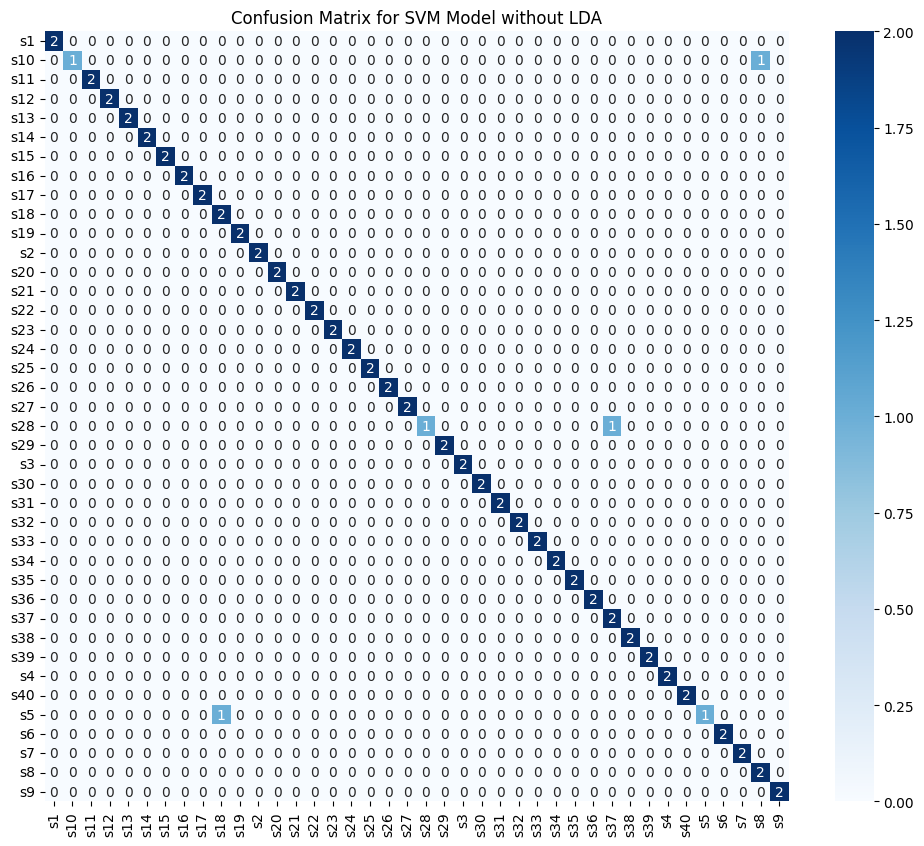
\includegraphics[width=0.8\textwidth]{output_05.png}
\end{center}


\textbf{AI-Generated}

\begin{lstlisting}[language=Python]
import numpy as np
from sklearn.datasets import fetch_olivetti_faces
from sklearn.model_selection import train_test_split
from sklearn.preprocessing import StandardScaler
from sklearn.discriminant_analysis import LinearDiscriminantAnalysis
from sklearn.svm import SVC
from sklearn.metrics import classification_report, accuracy_score, confusion_matrix
import matplotlib.pyplot as plt
import seaborn as sns

# Step 1: Load the ORL Dataset
data = fetch_olivetti_faces()
X = data.data  # 400 samples, 4096 features (64x64 images)
y = data.target  # 40 classes (subjects)

print(f"Dataset shape: {X.shape}, Labels shape: {y.shape}")

# Step 2: Train-Test Split
X_train, X_test, y_train, y_test = train_test_split(
    X, y, test_size=0.3, random_state=42, stratify=y
)

# Step 3: Standardize features
scaler = StandardScaler()
X_train_std = scaler.fit_transform(X_train)
X_test_std = scaler.transform(X_test)

# Step 4: Apply LDA
lda = LinearDiscriminantAnalysis(n_components=39)  # max components = n_classes - 1
X_train_lda = lda.fit_transform(X_train_std, y_train)
X_test_lda = lda.transform(X_test_std)

print(f"LDA-transformed shape: {X_train_lda.shape}")

# Step 5: Train Classifier (SVM)
classifier = SVC(kernel='linear', C=1, random_state=42)
classifier.fit(X_train_lda, y_train)

# Step 6: Predict and Analyze Performance
y_pred = classifier.predict(X_test_lda)

print("\nClassification Report:")
print(classification_report(y_test, y_pred))

print("Accuracy Score:", accuracy_score(y_test, y_pred))

# Step 7: Plot Confusion Matrix
conf_mat = confusion_matrix(y_test, y_pred)
plt.figure(figsize=(12, 10))
sns.heatmap(conf_mat, annot=False, cmap='Blues', xticklabels=False, yticklabels=False)
plt.title("Confusion Matrix")
plt.xlabel("Predicted")
plt.ylabel("True")
plt.show()
\end{lstlisting}

\vspace{1em}

\textbf{Comments on comparisons}

\begin{itemize}
    \item The AI generated code uses the built-in fetch\_olivetti\_faces function from scikit-learn to directly load the ORL dataset, while the code I have written manually loads images from a local directory, flattens them, and organizes them into training and testing folders. The manual approach gives more control over data preprocessing and file management.
    \item Both codes apply Linear Discriminant Analysis (LDA) for dimensionality reduction and use a linear SVM for classification. However, the code I have written goes a step further by also training and evaluating an SVM on the original (non-LDA) features, showing a comparison of performance with and without LDA.
\end{itemize}

\textbf{Results}
\begin{lstlisting}[language=Python]
downloading Olivetti faces from https://ndownloader.figshare.com/files/5976027 to /home/hrishikesh/scikit_learn_data
Dataset shape: (400, 4096), Labels shape: (400,)
LDA-transformed shape: (280, 39)

Classification Report:
              precision    recall  f1-score   support

           0       1.00      1.00      1.00         3
           1       1.00      1.00      1.00         3
           2       1.00      1.00      1.00         3
           3       1.00      1.00      1.00         3
           4       1.00      1.00      1.00         3
           5       1.00      1.00      1.00         3
           6       1.00      1.00      1.00         3
           7       1.00      1.00      1.00         3
           8       1.00      1.00      1.00         3
           9       1.00      0.67      0.80         3
          10       1.00      1.00      1.00         3
          11       1.00      1.00      1.00         3
          12       1.00      1.00      1.00         3
          13       1.00      1.00      1.00         3
          14       1.00      1.00      1.00         3
          15       1.00      1.00      1.00         3
          16       1.00      1.00      1.00         3
          17       1.00      1.00      1.00         3
...
   macro avg       0.99      0.98      0.98       120
weighted avg       0.99      0.98      0.98       120

Accuracy Score: 0.9833333333333333

\end{lstlisting}

\textbf{Verified By}



\newpage

\section*{Cycle II}
\begin{center}
\textbf{Experiment 2}
\label{exp2}
\end{center}

\vspace{1em}

\raggedright{
  \textbf{Problem}\par
  \noindent
  Use PCA to reduce the dimensionality of an image dataset and apply KNN for classification\par
}


\vspace{1em}

\textbf{Aim and Objectives}

To use PCA for reducing the dimensionality of an image dataset and apply KNN for classification, including data preprocessing, feature reduction, model training, and performance evaluation.

\vspace{1em}

\textbf{Program Code}

\begin{lstlisting}[language=Python]
import cupy as cp
from cuml.decomposition import PCA
from cuml.neighbors import KNeighborsClassifier
from cuml.preprocessing import LabelEncoder, StandardScaler
from cuml.metrics import accuracy_score, confusion_matrix
from sklearn.metrics import classification_report
from cuml.preprocessing import StandardScaler
import seaborn as sns
import cudf as df
import matplotlib.pyplot as plt
\end{lstlisting}

\begin{lstlisting}[language=Python]
Here we are going to take the MNIST dataset
\end{lstlisting}

\begin{lstlisting}[language=Python]
train_set = df.read_csv("../datasets/mnist_train.csv")
test_set = df.read_csv("../datasets/mnist_test.csv")
\end{lstlisting}

\begin{lstlisting}[language=Python]
train_set
\end{lstlisting}

\begin{center}
  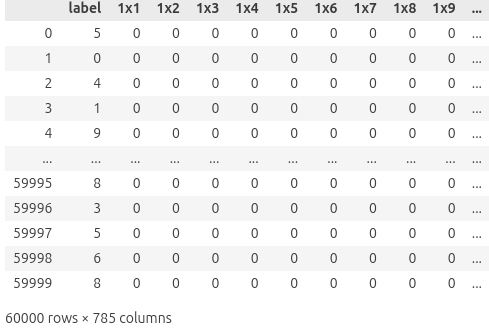
\includegraphics[width=0.5\textwidth]{output_II_01.png}
\end{center}

\begin{lstlisting}[language=Python]
train_set.describe()
\end{lstlisting}

\begin{lstlisting}[language=Python]
plt.subplots(1, 10, figsize=(20, 17))
for i in range(10):
    plt.subplot(1, 10, i + 1)
    image = train_set[train_set["label"] == i].to_numpy()[0][1:].reshape(28, 28)
    plt.imshow(image, cmap="gray")
    plt.axis("off")
    plt.title(i)
plt.show()
\end{lstlisting}

\begin{center}
  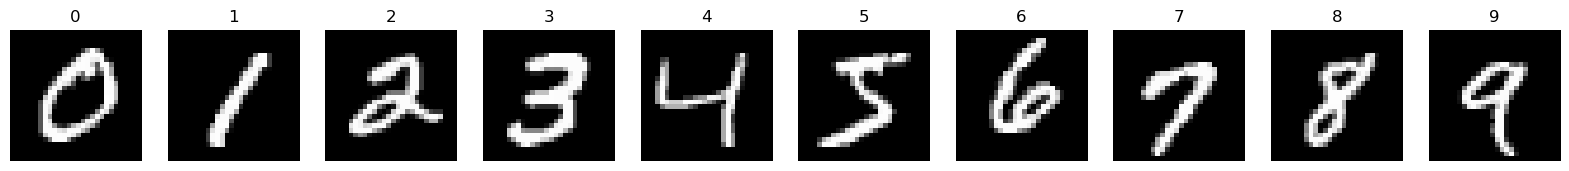
\includegraphics[width=1.0\textwidth]{output_II_03.png}
\end{center}

\begin{lstlisting}[language=Python]
for i in range(10):
    print(f"Number of {i} in train set: {train_set[train_set['label'] == i].shape[0]}")
    print(f"Number of {i} in test set: {test_set[test_set['label'] == i].shape[0]}")
\end{lstlisting}

\begin{lstlisting}[language=Python]
Number of 0 in train set: 5923
Number of 0 in test set: 980
Number of 1 in train set: 6742
Number of 1 in test set: 1135
Number of 2 in train set: 5958
Number of 2 in test set: 1032
Number of 3 in train set: 6131
Number of 3 in test set: 1010
Number of 4 in train set: 5842
Number of 4 in test set: 982
Number of 5 in train set: 5421
Number of 5 in test set: 892
Number of 6 in train set: 5918
Number of 6 in test set: 958
Number of 7 in train set: 6265
Number of 7 in test set: 1028
Number of 8 in train set: 5851
Number of 8 in test set: 974
Number of 9 in train set: 5949
Number of 9 in test set: 1009
\end{lstlisting}

\begin{lstlisting}[language=Python]
X_train = train_set.drop("label", axis=1).to_cupy()
y_train = train_set["label"].to_cupy()
X_test = test_set.drop("label", axis=1).to_cupy()
y_test = test_set["label"].to_cupy()
\end{lstlisting}

\begin{lstlisting}[language=Python]
std_scaler = StandardScaler()
X_train = std_scaler.fit_transform(X_train)
X_test = std_scaler.transform(X_test)
\end{lstlisting}

\begin{lstlisting}[language=Python]
pca = PCA(n_components=39)
X_train = pca.fit_transform(X_train)
X_test = pca.transform(X_test)
\end{lstlisting}

\begin{lstlisting}[language=Python]
Training a KNN classifier on the PCA applied dataset
\end{lstlisting}

\begin{lstlisting}[language=Python]
knn_01 = KNeighborsClassifier(n_neighbors = 5)
knn_01.fit(X_train, y_train)
\end{lstlisting}

\begin{center}
  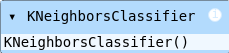
\includegraphics[width=0.3\textwidth]{output_II_04.png}
\end{center}

\begin{lstlisting}[language=Python]
pred_01 = knn_01.predict(X_test)
\end{lstlisting}

\begin{lstlisting}[language=Python]
print("Accuracy:", accuracy_score(y_test, pred_01))
conf_matrix = confusion_matrix(y_test, pred_01)

sns.heatmap(conf_matrix.get(), annot=True, fmt="d", cmap="Blues", xticklabels=range(10), yticklabels=range(10))
plt.xlabel("Predicted")
plt.ylabel("Actual")
plt.title("Confusion Matrix")
plt.show()
\end{lstlisting}

\begin{lstlisting}[language=Python]
  Accuracy: 0.9581
\end{lstlisting}

\begin{center}
  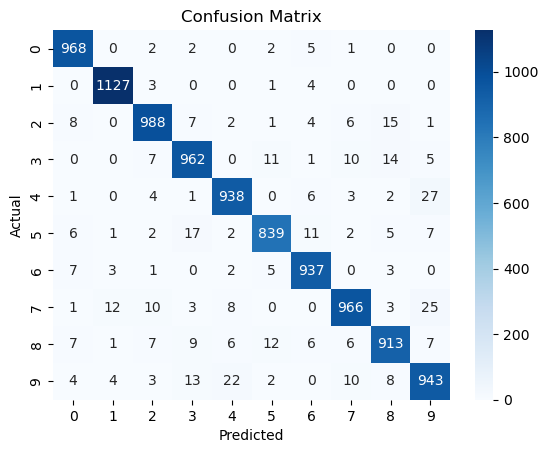
\includegraphics[width=0.7\textwidth]{output_II_05.png}
\end{center}

\begin{lstlisting}[language=Python]
print(classification_report(y_test.get(), pred_01.get()))
\end{lstlisting}

\begin{lstlisting}[language=Python]
              precision    recall  f1-score   support

           0       0.97      0.99      0.98       980
           1       0.98      0.99      0.99      1135
           2       0.96      0.96      0.96      1032
           3       0.95      0.95      0.95      1010
           4       0.96      0.96      0.96       982
           5       0.96      0.94      0.95       892
           6       0.96      0.98      0.97       958
           7       0.96      0.94      0.95      1028
           8       0.95      0.94      0.94       974
           9       0.93      0.93      0.93      1009

    accuracy                           0.96     10000
   macro avg       0.96      0.96      0.96     10000
weighted avg       0.96      0.96      0.96     10000

\end{lstlisting}

\vspace{1em}
\textbf{AI-Generated}

\begin{lstlisting}[language=Python]
import numpy as np
from sklearn.datasets import fetch_olivetti_faces
from sklearn.model_selection import train_test_split
from sklearn.preprocessing import StandardScaler
from sklearn.discriminant_analysis import LinearDiscriminantAnalysis
from sklearn.svm import SVC
from sklearn.metrics import classification_report, accuracy_score, confusion_matrix
import matplotlib.pyplot as plt
import seaborn as sns

# Step 1: Load the ORL Dataset
data = fetch_olivetti_faces()
X = data.data  # 400 samples, 4096 features (64x64 images)
y = data.target  # 40 classes (subjects)

print(f"Dataset shape: {X.shape}, Labels shape: {y.shape}")

# Step 2: Train-Test Split
X_train, X_test, y_train, y_test = train_test_split(
    X, y, test_size=0.3, random_state=42, stratify=y
)

# Step 3: Standardize features
scaler = StandardScaler()
X_train_std = scaler.fit_transform(X_train)
X_test_std = scaler.transform(X_test)

# Step 4: Apply LDA
lda = LinearDiscriminantAnalysis(n_components=39)  # max components = n_classes - 1
X_train_lda = lda.fit_transform(X_train_std, y_train)
X_test_lda = lda.transform(X_test_std)

print(f"LDA-transformed shape: {X_train_lda.shape}")

# Step 5: Train Classifier (SVM)
classifier = SVC(kernel='linear', C=1, random_state=42)
classifier.fit(X_train_lda, y_train)

# Step 6: Predict and Analyze Performance
y_pred = classifier.predict(X_test_lda)

print("\nClassification Report:")
print(classification_report(y_test, y_pred))

print("Accuracy Score:", accuracy_score(y_test, y_pred))

# Step 7: Plot Confusion Matrix
conf_mat = confusion_matrix(y_test, y_pred)
plt.figure(figsize=(12, 10))
sns.heatmap(conf_mat, annot=False, cmap='Blues', xticklabels=False, yticklabels=False)
plt.title("Confusion Matrix")
plt.xlabel("Predicted")
plt.ylabel("True")
plt.show()
\end{lstlisting}

\vspace{1em}

\textbf{Comments on comparisons}

\begin{itemize}
    \item The AI generated code has used sklearn which is a cpu based library compared to the code I have written which uses cuml, a GPU accelerated library.
    \item Both follow the same workflow—data preprocessing, PCA, KNN classification, and evaluation—but differ in dataset
\end{itemize}
\vspace{1em}

\textbf{Results}

\begin{lstlisting}[language=Python]
Dataset shape: (400, 4096), Number of classes: 40
PCA-reduced shape: (280, 100)

Classification Report:
              precision    recall  f1-score   support

           0       0.50      0.33      0.40         3
           1       1.00      0.67      0.80         3
           2       1.00      0.67      0.80         3
           3       1.00      0.33      0.50         3
           4       0.40      0.67      0.50         3
           5       0.50      1.00      0.67         3
           6       1.00      1.00      1.00         3
           7       1.00      0.33      0.50         3
           8       1.00      1.00      1.00         3
           9       1.00      0.67      0.80         3
          10       1.00      1.00      1.00         3
          11       1.00      0.67      0.80         3
          12       1.00      0.33      0.50         3
          13       1.00      1.00      1.00         3
          14       0.30      1.00      0.46         3
          15       0.00      0.00      0.00         3
          16       1.00      0.33      0.50         3
          17       0.67      0.67      0.67         3
          18       1.00      1.00      1.00         3
...
   macro avg       0.76      0.69      0.67       120
weighted avg       0.76      0.69      0.67       120

Accuracy: 0.6916666666666667
\end{lstlisting}

\begin{center}
  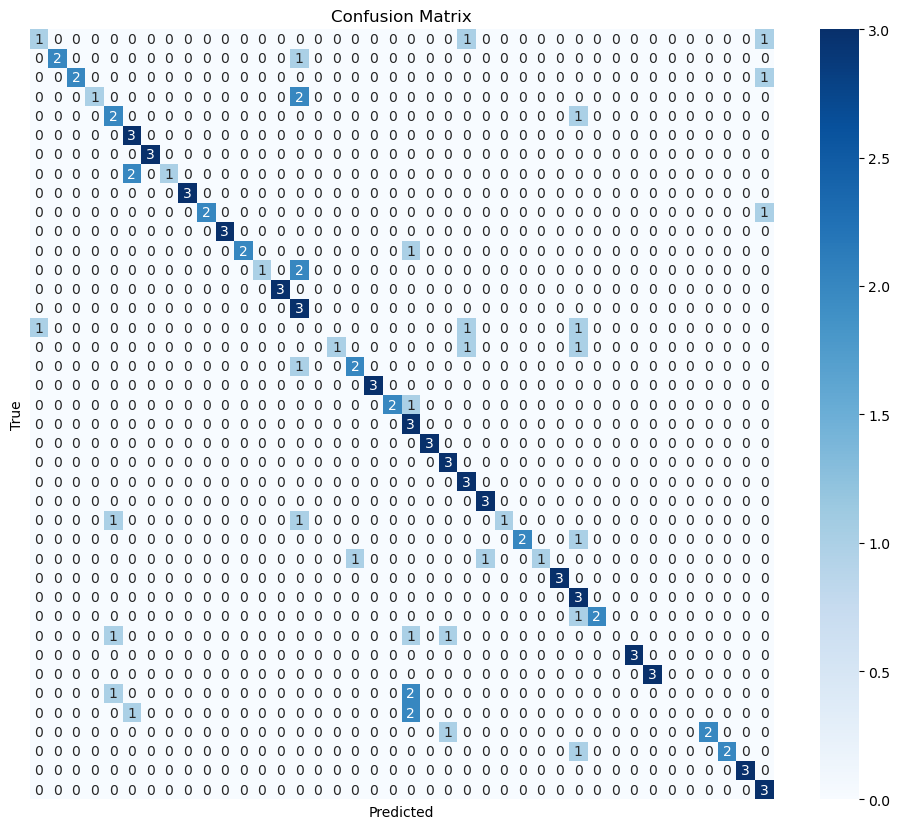
\includegraphics[width=0.7\textwidth]{output_II_06.png}
\end{center}

\textbf{Verified By}

\newpage

\section*{Cycle II}
\begin{center}
\textbf{Experiment 3}
\label{exp3}
\end{center}

\vspace{1em}

\raggedright{
  \textbf{Problem}\par
  \noindent
  Perform exploratory data analysis (EDA) on Iris dataset to understand its structure. Apply Principal Component Analysis (PCA) for dimensionality reduction. Visualize the transformed dataset and analyze the effectiveness of PCA in reducing the dimensions.\par
}


\vspace{1em}

\textbf{Aim and Objectives}

To explore the Iris dataset and apply PCA for dimensionality reduction, followed by visualization and analysis of the transformed data to assess PCA’s effectiveness.

\vspace{1em}

\textbf{Program Code}

\begin{lstlisting}[language=Python]
import pandas as pd
from sklearn.model_selection import train_test_split
from sklearn.decomposition import PCA
from sklearn.preprocessing import StandardScaler
from sklearn.linear_model import LogisticRegression
from sklearn.metrics import accuracy_score, confusion_matrix, classification_report
import seaborn as sns
import matplotlib.pyplot as plt
\end{lstlisting}

\begin{lstlisting}[language=Python]
iris = pd.read_csv("../datasets/Iris.csv")
\end{lstlisting}

\begin{lstlisting}[language=Python]
iris
\end{lstlisting}

\begin{center}
  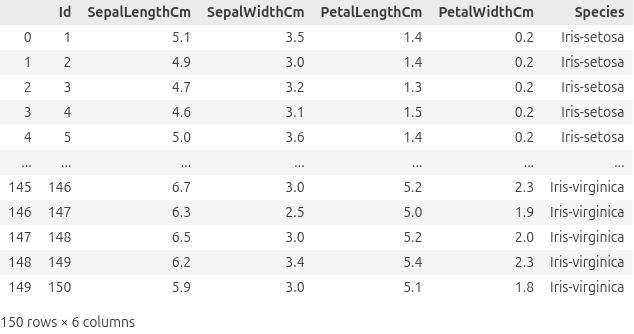
\includegraphics[width=0.65\textwidth]{output_II_07.png}
\end{center}

\begin{lstlisting}[language=Python]
iris.describe()
\end{lstlisting}

\begin{center}
  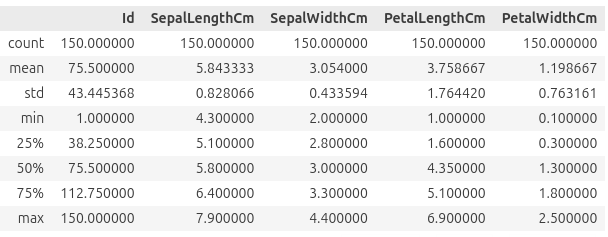
\includegraphics[width=0.65\textwidth]{output_II_08.png}
\end{center}


\begin{lstlisting}[language=Python]
iris_X = iris.drop(columns=["Id", "Species"])
iris_y = iris["Species"]
\end{lstlisting}

\begin{lstlisting}[language=Python]
for column in iris_X.columns:
    q1 = iris_X[column].quantile(0.25)
    q3 = iris_X[column].quantile(0.75)
    iqr = q3 - q1

    bin_width = 2 * iqr / (len(iris_X) ** (1 / 3))

    bins = int((iris_X[column].max() - iris_X[column].min()) / bin_width)
    plt.figure(figsize=(6, 6))
    sns.histplot(iris_X[column], bins=bins, kde=True)
    plt.title(f"Histogram of {column}")
    plt.xlabel(column)
    plt.ylabel("Frequency")
    plt.tight_layout()
    plt.show()

\end{lstlisting}

\begin{center}
  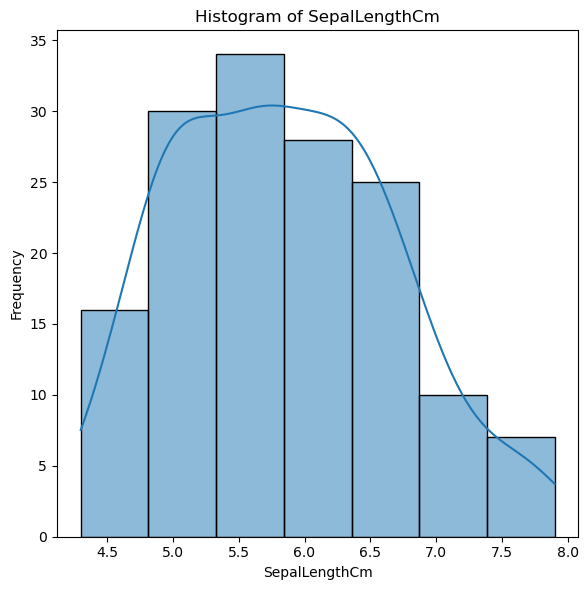
\includegraphics[width=0.5\textwidth]{output_II_09.png}
  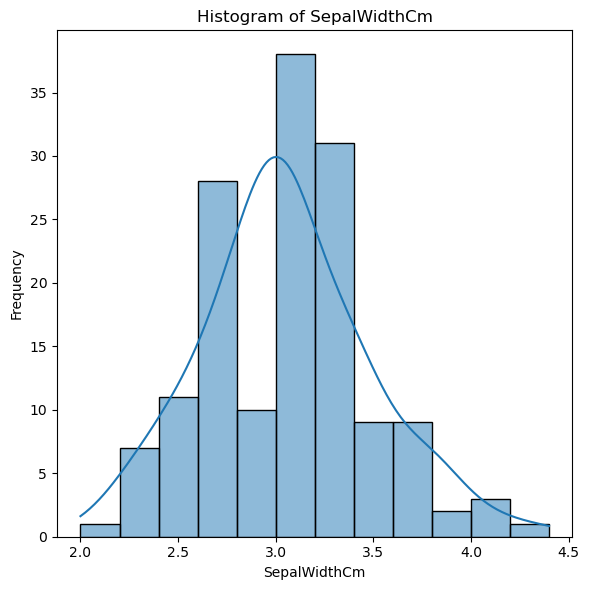
\includegraphics[width=0.5\textwidth]{output_II_10.png}
  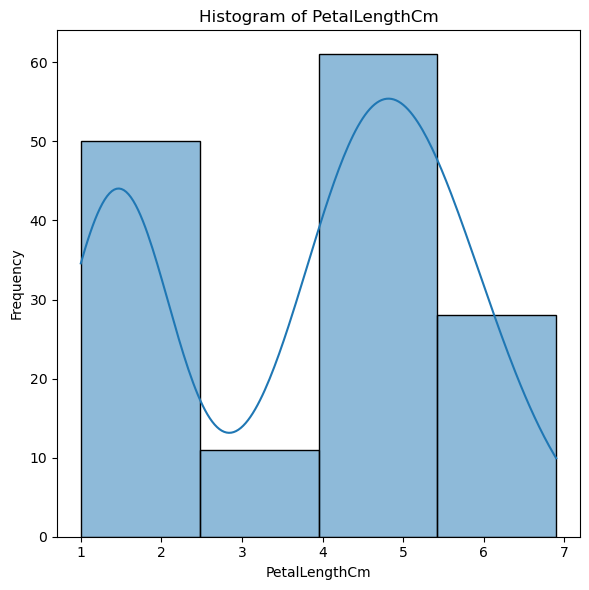
\includegraphics[width=0.5\textwidth]{output_II_11.png}
  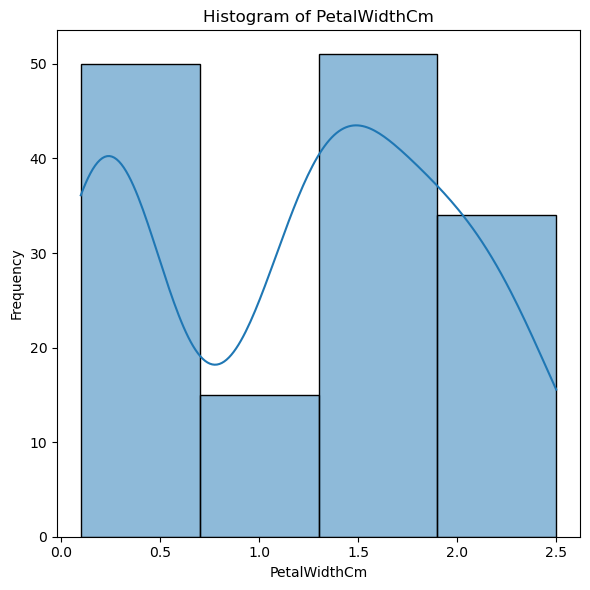
\includegraphics[width=0.5\textwidth]{output_II_12.png}
\end{center}

\begin{lstlisting}[language=Python]
corr = iris_X.corr()
plt.figure(figsize=(7, 5))
sns.heatmap(corr, annot=True, cmap="coolwarm", fmt=".2f", square=True, cbar_kws={"shrink": .8})
plt.title("Correlation Matrix")
plt.tight_layout()
plt.show()
\end{lstlisting}

\begin{center}
  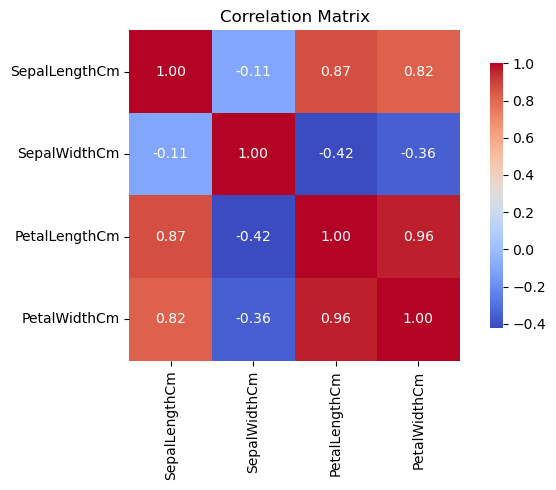
\includegraphics[width=0.6\textwidth]{output_II_13.png}
\end{center}

\begin{lstlisting}[language=Python]
for column in iris_X.columns:
    plt.figure(figsize=(5, 2))
    sns.boxplot(x=iris[column])
    plt.title(f'Boxplot of {column}')
    plt.xlabel(column)
    plt.show()
\end{lstlisting}

\begin{center}
  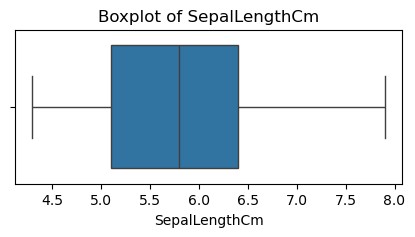
\includegraphics[width=0.5\textwidth]{output_II_14.png}
  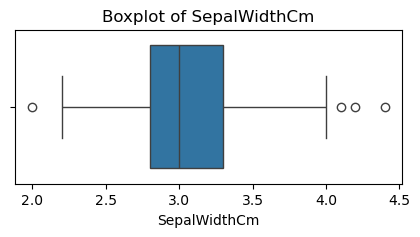
\includegraphics[width=0.5\textwidth]{output_II_15.png}
  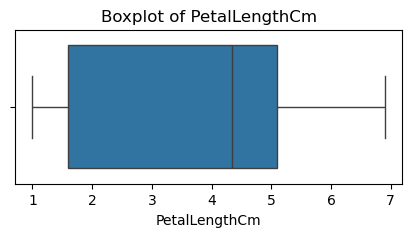
\includegraphics[width=0.5\textwidth]{output_II_16.png}
  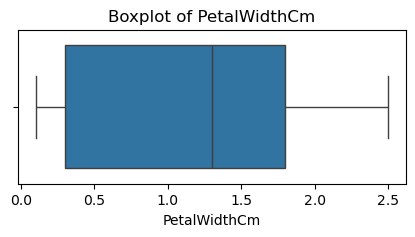
\includegraphics[width=0.5\textwidth]{output_II_17.png}
\end{center}

\begin{lstlisting}[language=Python]
sns.pairplot(iris, hue="Species", markers=["o", "s", "D"], palette="Set2")
\end{lstlisting}

\begin{center}
  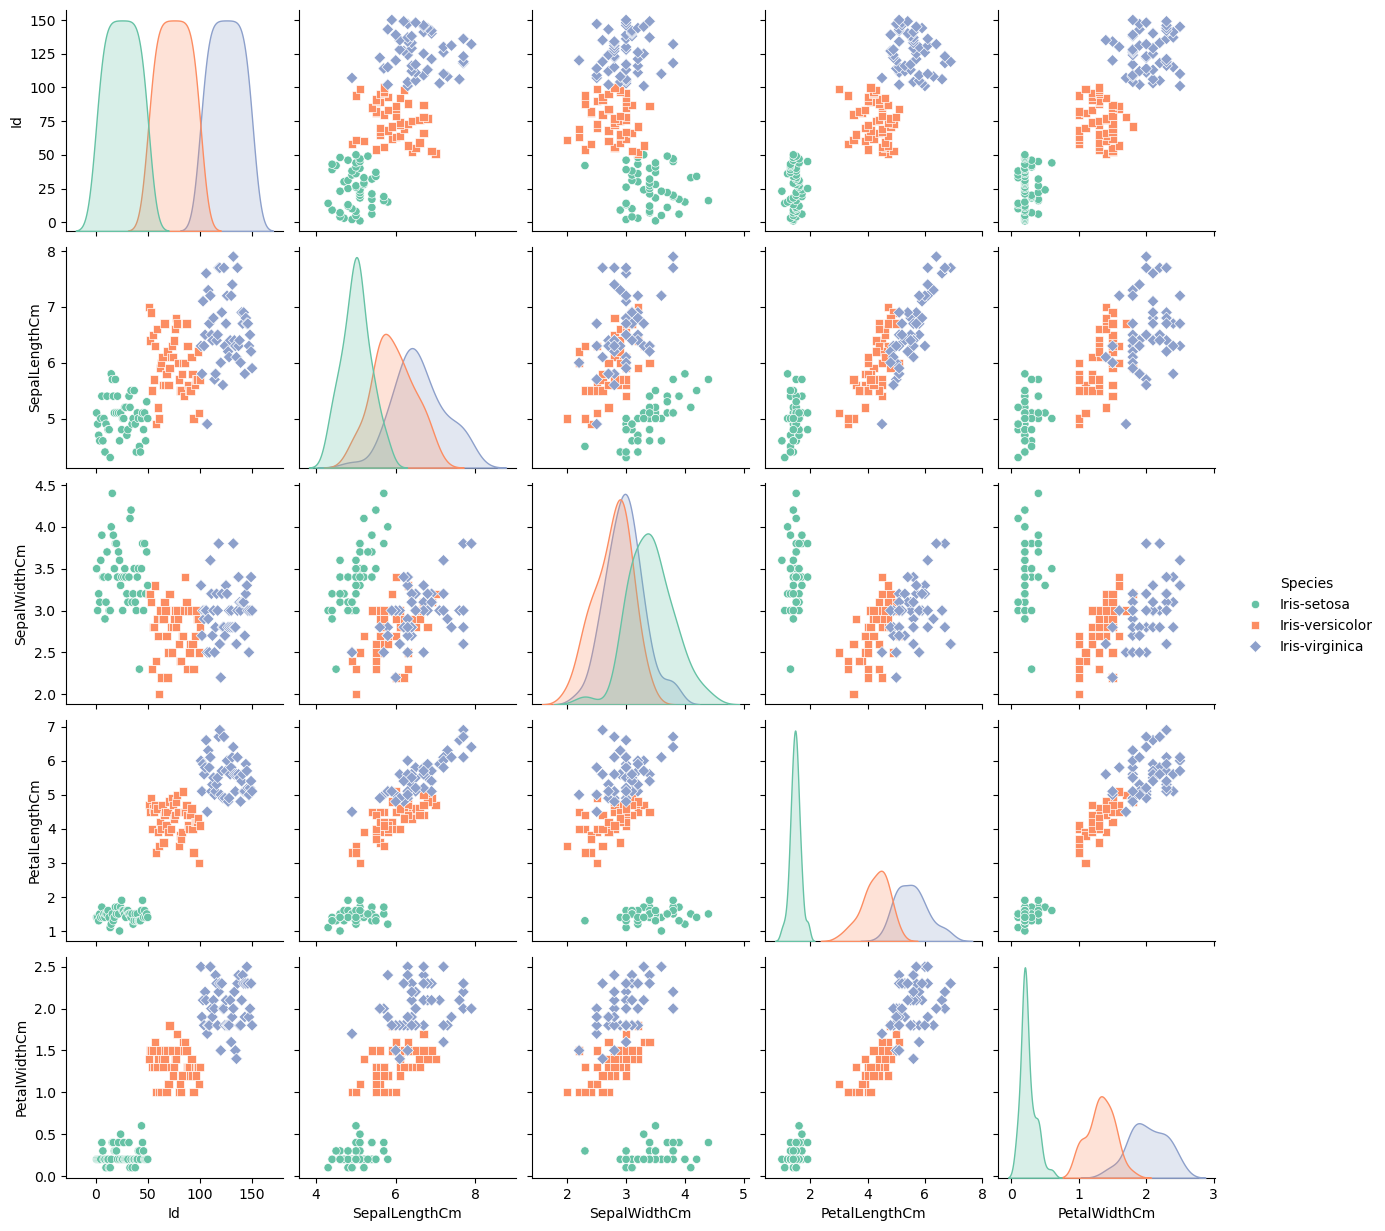
\includegraphics[width=1.07\textwidth]{output_II_18.png}
\end{center}


\begin{lstlisting}[language=Python]
X_train, X_test, y_train, y_test = train_test_split(iris_X, iris_y, test_size=0.2, random_state=42)
\end{lstlisting}

\begin{lstlisting}[language=Python]
pca = PCA(n_components=2)
X_train_pca = pca.fit_transform(X_train)
X_test_pca = pca.transform(X_test)
\end{lstlisting}

\begin{lstlisting}[language=Python]
explained_variance = pca.explained_variance_ratio_
print(f"Explained variance by PCA components: {explained_variance}")
plt.figure(figsize=(8, 6))
sns.scatterplot(x=X_train_pca[:, 0], y=X_train_pca[:, 1], hue=y_train, palette="Set2")
plt.title("PCA of Iris Dataset")
plt.xlabel("Principal Component 1")
plt.ylabel("Principal Component 2")
\end{lstlisting}

\begin{lstlisting}[language=Python]
Explained variance by PCA components: [0.9195717  0.05707944]
\end{lstlisting}

\begin{center}
  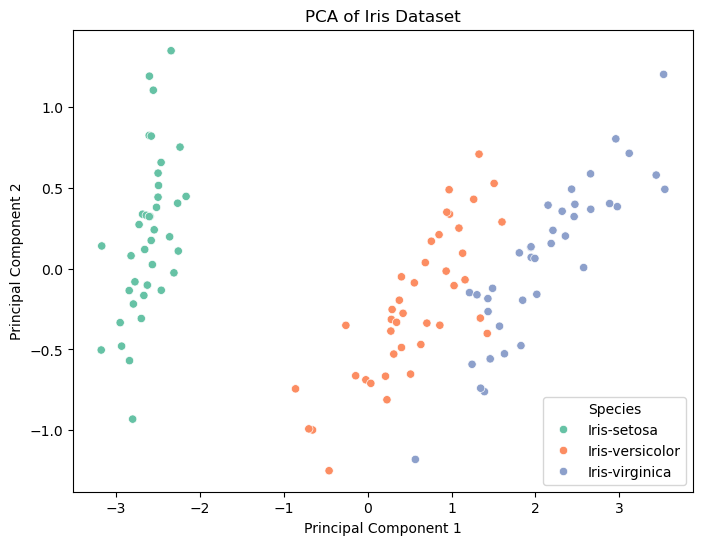
\includegraphics[width=1.07\textwidth]{output_II_19.png}
\end{center}

\begin{lstlisting}[language=Python]
x = [f"PC{i}" for i in range(1, len(pca.explained_variance_ratio_) + 1)]
sns.barplot(x=x, y=explained_variance)
\end{lstlisting}

\begin{center}
  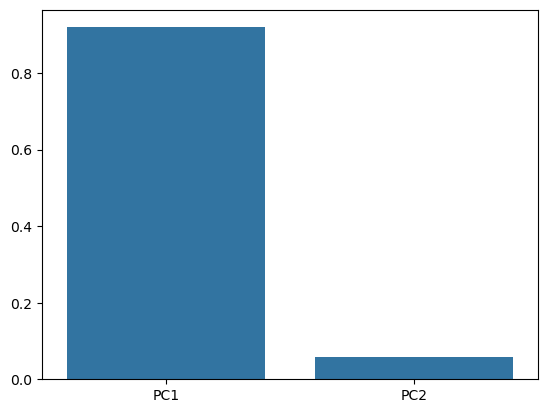
\includegraphics[width=0.5\textwidth]{output_II_20.png}
\end{center}

\begin{lstlisting}[language=Python]
log_model = LogisticRegression(solver='newton-cholesky')
\end{lstlisting}

\begin{lstlisting}[language=Python]
log_model.fit(X_train_pca, y_train)
\end{lstlisting}

\begin{center}
  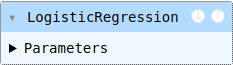
\includegraphics[width=0.25\textwidth]{output_II_21.png}
\end{center}

\begin{lstlisting}[language=Python]
pred_01 = log_model.predict(X_test_pca)
accuracy = accuracy_score(y_test, pred_01)
print("Accuracy:", accuracy)
conf_matrix = confusion_matrix(y_test, pred_01)
print("Classification Report:\n", classification_report(y_test, pred_01))
plt.figure(figsize=(8, 6))
sns.heatmap(conf_matrix, annot=True, fmt='d', cmap='Blues',
            xticklabels=iris_y.unique(), yticklabels=iris_y.unique())
plt.title('Confusion Matrix')
plt.xlabel('Predicted')
plt.ylabel('Actual')
plt.tight_layout()
plt.show()
\end{lstlisting}

\begin{lstlisting}[language=Python]
Accuracy: 1.0
Classification Report:
                  precision    recall  f1-score   support

    Iris-setosa       1.00      1.00      1.00        10
Iris-versicolor       1.00      1.00      1.00         9
 Iris-virginica       1.00      1.00      1.00        11

       accuracy                           1.00        30
      macro avg       1.00      1.00      1.00        30
   weighted avg       1.00      1.00      1.00        30
\end{lstlisting}

\begin{center}
  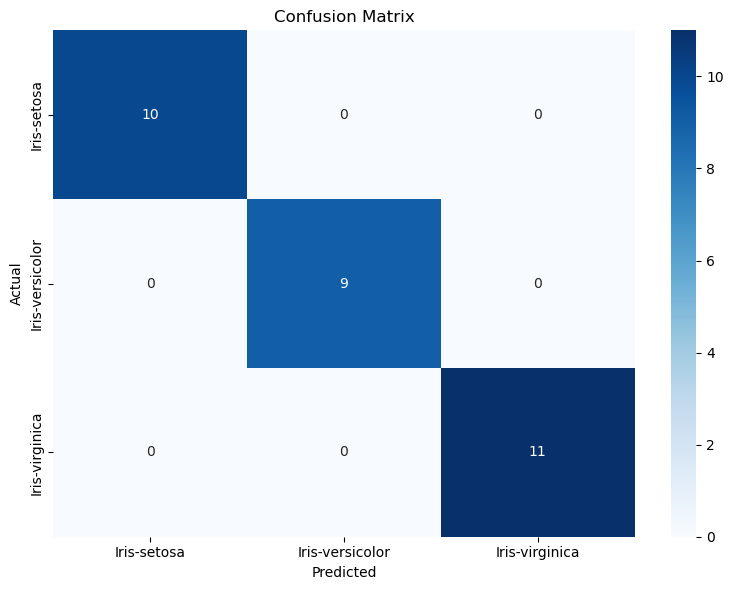
\includegraphics[width=0.6\textwidth]{output_II_22.png}
\end{center}

\begin{lstlisting}[language=Python]
  log_model_02 = LogisticRegression(solver='newton-cholesky')
  log_model_02.fit(X_train, y_train)
\end{lstlisting}

\begin{center}
  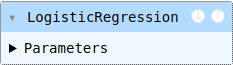
\includegraphics[width=0.25\textwidth]{output_II_21.png}
\end{center}

\begin{lstlisting}[language=Python]
accuracy_02 = accuracy_score(y_test, log_model_02.predict(X_test))
print("Accuracy without PCA:", accuracy_02)
conf_matrix_02 = confusion_matrix(y_test, log_model_02.predict(X_test))
print("Classification Report without PCA:\n", classification_report(y_test, log_model_02.predict(X_test)))
plt.figure(figsize=(8, 6))
sns.heatmap(conf_matrix_02, annot=True, fmt='d', cmap='Blues',
            xticklabels=iris_y.unique(), yticklabels=iris_y.unique())
plt.title('Confusion Matrix without PCA')
plt.xlabel('Predicted')
plt.ylabel('Actual')
plt.tight_layout()
\end{lstlisting}

\begin{lstlisting}[language=Python]
Accuracy without PCA: 1.0
Classification Report without PCA:
                  precision    recall  f1-score   support

    Iris-setosa       1.00      1.00      1.00        10
Iris-versicolor       1.00      1.00      1.00         9
 Iris-virginica       1.00      1.00      1.00        11

       accuracy                           1.00        30
      macro avg       1.00      1.00      1.00        30
   weighted avg       1.00      1.00      1.00        30
\end{lstlisting}

\begin{center}
  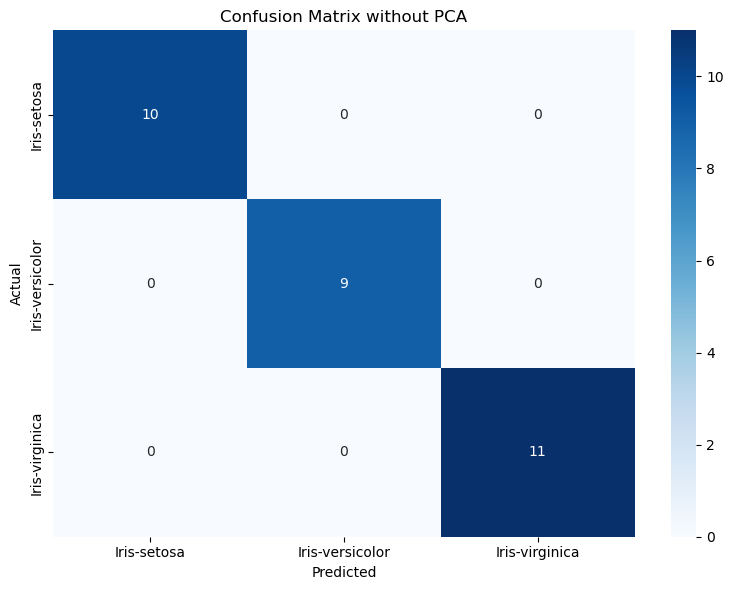
\includegraphics[width=0.6\textwidth]{output_II_23.png}
\end{center}


\vspace{1em}
\textbf{AI-Generated}

\begin{lstlisting}[language=Python]
import numpy as np
import pandas as pd
import seaborn as sns
import matplotlib.pyplot as plt

from sklearn.datasets import load_iris
from sklearn.preprocessing import StandardScaler
from sklearn.decomposition import PCA
from mpl_toolkits.mplot3d import Axes3D

# Step 1: Load the Iris dataset
iris = load_iris()
X = pd.DataFrame(iris.data, columns=iris.feature_names)
y = pd.Series(iris.target, name='species')
species_names = iris.target_names

# Combine features and target for easier EDA
df = pd.concat([X, y], axis=1)

# Step 2: EDA
print("Basic Info:")
print(df.info(), "\n")

print("Descriptive Statistics:")
print(df.describe(), "\n")

print("Value Counts:")
print(df['species'].value_counts(), "\n")

# Pairplot
sns.pairplot(df, hue="species", palette='Set2')
plt.suptitle("Pairplot of Iris Features", y=1.02)
plt.show()

# Correlation heatmap
plt.figure(figsize=(8, 6))
sns.heatmap(X.corr(), annot=True, cmap='coolwarm')
plt.title("Feature Correlation Matrix")
plt.show()

# Step 3: Standardize the data
scaler = StandardScaler()
X_scaled = scaler.fit_transform(X)

# Step 4: Apply PCA
pca = PCA()
X_pca = pca.fit_transform(X_scaled)

# Explained variance
explained_var = pca.explained_variance_ratio_
cum_var = np.cumsum(explained_var)

# Plot explained variance
plt.figure(figsize=(8, 5))
plt.bar(range(1, len(explained_var)+1), explained_var, alpha=0.7, label='Individual')
plt.plot(range(1, len(cum_var)+1), cum_var, marker='o', color='red', label='Cumulative')
plt.xticks(range(1, len(explained_var)+1))
plt.ylabel('Explained Variance Ratio')
plt.xlabel('Principal Component')
plt.title('Explained Variance by PCA Components')
plt.legend()
plt.grid(True)
plt.show()

# Step 5: Visualize the transformed data (2D)
pca_2d = PCA(n_components=2)
X_2d = pca_2d.fit_transform(X_scaled)

plt.figure(figsize=(8, 6))
sns.scatterplot(x=X_2d[:, 0], y=X_2d[:, 1], hue=species_names[y], palette='Set2')
plt.xlabel('PC1')
plt.ylabel('PC2')
plt.title('PCA: 2D Projection of Iris Dataset')
plt.legend(title='Species')
plt.grid(True)
plt.show()

# Step 6: Optional 3D Visualization
pca_3d = PCA(n_components=3)
X_3d = pca_3d.fit_transform(X_scaled)

fig = plt.figure(figsize=(10, 7))
ax = fig.add_subplot(111, projection='3d')
scatter = ax.scatter(X_3d[:, 0], X_3d[:, 1], X_3d[:, 2], c=y, cmap='Set2', edgecolor='k')
ax.set_title("PCA: 3D Projection of Iris Dataset")
ax.set_xlabel("PC1")
ax.set_ylabel("PC2")
ax.set_zlabel("PC3")
# plt.legend(handles=scatter.legend_elements()[0], labels=species_names, title="Species")
plt.show()

# Step 7: PCA Effectiveness Summary
print("PCA Explained Variance Ratios:")
for i, ratio in enumerate(explained_var):
    print(f"  PC{i+1}: {ratio:.4f}")

print("\nCumulative Variance (first 2 PCs): {:.2f}%".format(cum_var[1] * 100))

\end{lstlisting}

\vspace{1em}

\textbf{Comments on comparisons}

\begin{itemize}
    \item The AI generated code has performed EDA and PCA on the iris dataset, fetched using the built-in load\_iris function from scikit-learn, while the code I have written uses a CSV file to load the dataset.
    \item The AI code uses PCA to reduce the dataset to 2D and 3D visualizations, while my code applies PCA to reduce the dataset to 2 components and uses logistic regression for classification and comparison of performance with and without PCA.
\end{itemize}
\vspace{1em}

\textbf{Results}

\begin{lstlisting}[language=Python]
  Basic Info:
  <class 'pandas.core.frame.DataFrame'>
  RangeIndex: 150 entries, 0 to 149
  Data columns (total 5 columns):
  #   Column             Non-Null Count  Dtype  
  ---  ------             --------------  -----  
  0   sepal length (cm)  150 non-null    float64
  1   sepal width (cm)   150 non-null    float64
  2   petal length (cm)  150 non-null    float64
  3   petal width (cm)   150 non-null    float64
  4   species            150 non-null    int64  
  dtypes: float64(4), int64(1)
  memory usage: 6.0 KB
  None 
  
  Descriptive Statistics:
  sepal length (cm)  sepal width (cm)  petal length (cm)  \
  count         150.000000        150.000000         150.000000   
  mean            5.843333          3.057333           3.758000   
  std             0.828066          0.435866           1.765298   
  min             4.300000          2.000000           1.000000   
  25%             5.100000          2.800000           1.600000   
  50%             5.800000          3.000000           4.350000   
  75%             6.400000          3.300000           5.100000   
  max             7.900000          4.400000           6.900000   
  ...
  1    50
  2    50
  Name: count, dtype: int64 
\end{lstlisting}

\begin{center}
  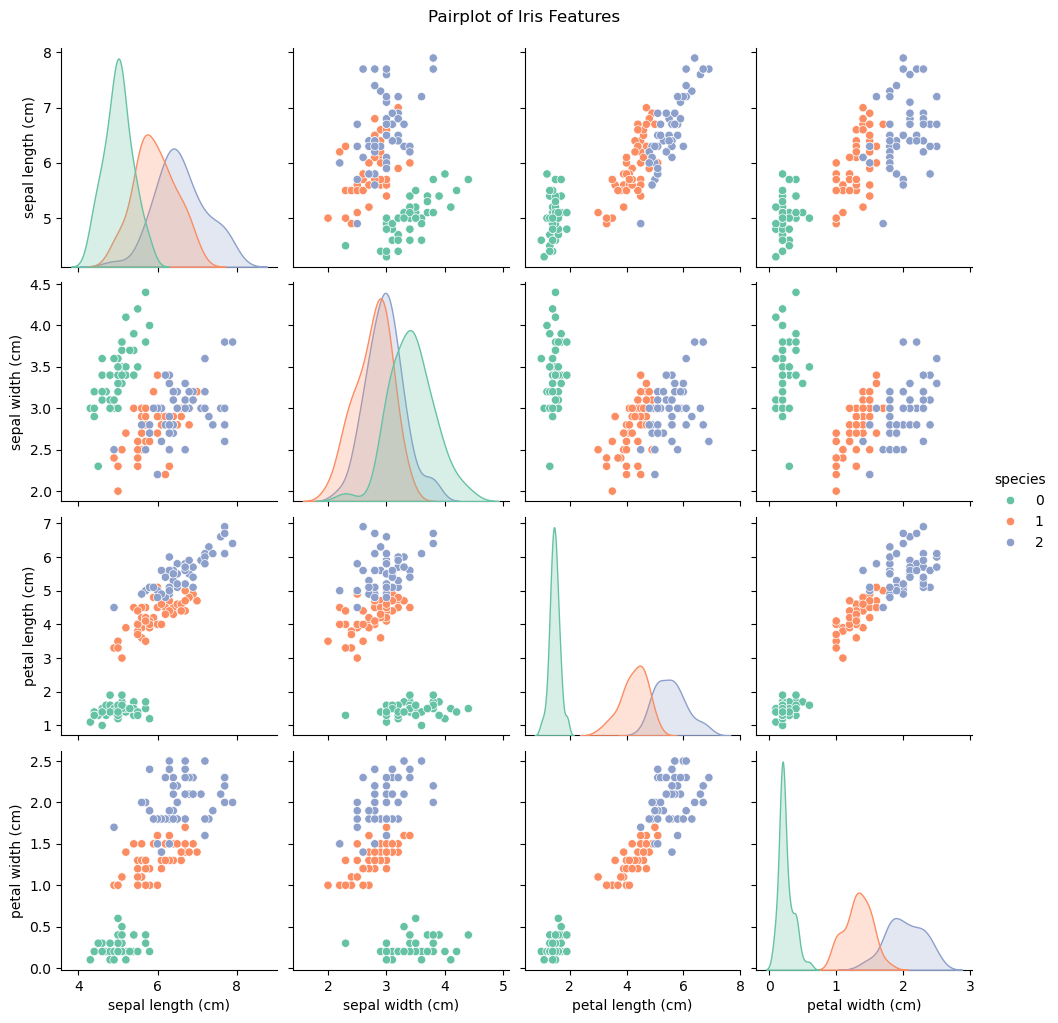
\includegraphics[width=0.7\textwidth]{output_II_24.png}
\end{center}
\begin{center}
  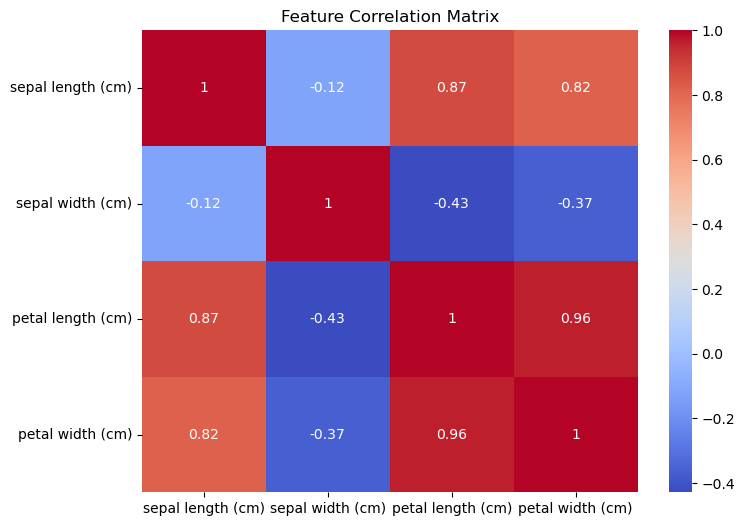
\includegraphics[width=0.7\textwidth]{output_II_25.png}
\end{center}
\begin{center}
  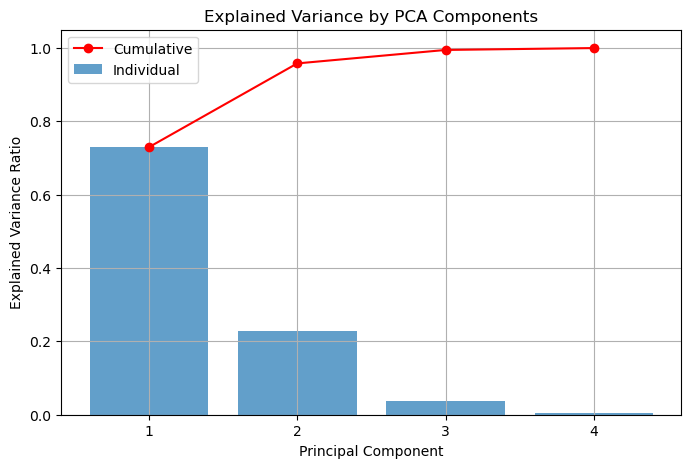
\includegraphics[width=0.7\textwidth]{output_II_26.png}
\end{center}
\begin{center}
  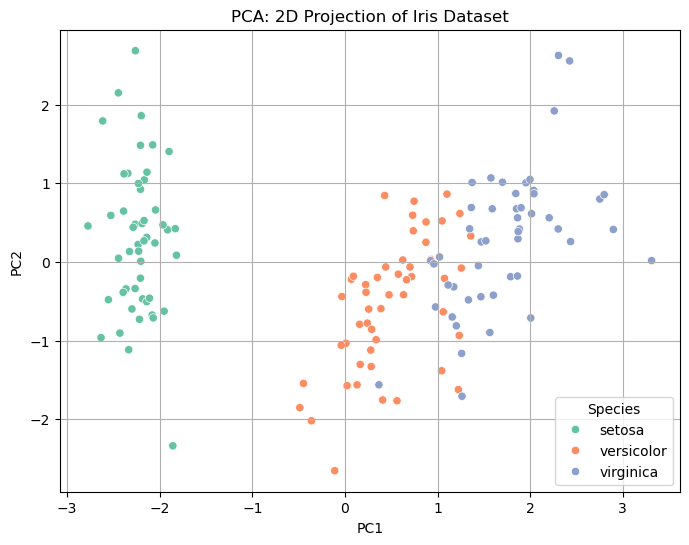
\includegraphics[width=0.7\textwidth]{output_II_27.png}
\end{center}
\begin{center}
  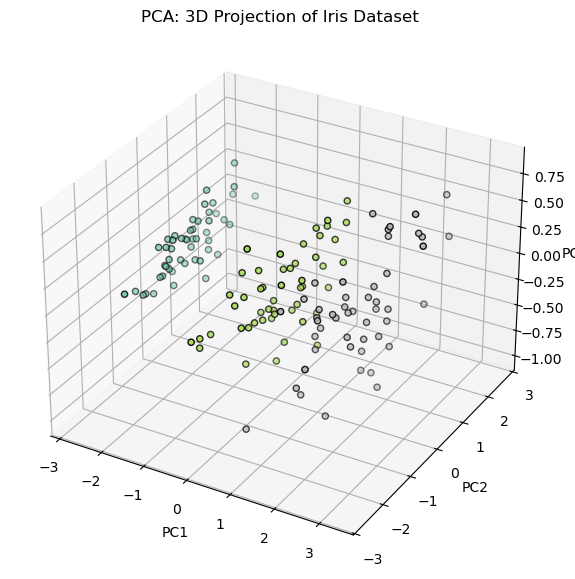
\includegraphics[width=0.7\textwidth]{output_II_28.png}
\end{center}

\begin{lstlisting}[language=Python]
PCA Explained Variance Ratios:
  PC1: 0.7296
  PC2: 0.2285
  PC3: 0.0367
  PC4: 0.0052

Cumulative Variance (first 2 PCs): 95.81%
\end{lstlisting}

\textbf{Verified By}

\newpage

\section*{Cycle II}
\begin{center}
\textbf{Experiment 4}
\label{exp4}
\end{center}

\vspace{1em}

\raggedright{
  \textbf{Problem}\par
  \noindent
  Implement a method to compute the Euclidean distance between two grayscale images.\par
}


\vspace{1em}

\textbf{Aim and Objectives}

To understand the concept of Euclidean distance and implement a method to compute it between two grayscale images, demonstrating the application of this metric in image processing.

\vspace{1em}

\textbf{Program Code}

\begin{lstlisting}[language=Python]
import cupy as cp
import cv2
import matplotlib.pyplot as plt
\end{lstlisting}

\begin{lstlisting}[language=Python]
def measure_euclid_dist(img_01, img_02):
    if img_01.shape != img_02.shape:
        img_02 = cv2.resize(img_02, (img_01.shape[1], img_01.shape[0]), interpolation=cv2.INTER_LINEAR)
    img_01 = img_01.flatten()
    img_02 = img_02.flatten()
    img_01 = cp.asarray(img_01, dtype=cp.float32)
    img_02 = cp.asarray(img_02, dtype=cp.float32)

    euclid = cp.linalg.norm(img_01 - img_02, axis=-1)

    euclid = cp.asnumpy(euclid)
    return euclid
\end{lstlisting}

\begin{lstlisting}[language=Python]
image_01 = cv2.imread("../images/scenery_01.jpg", cv2.IMREAD_GRAYSCALE)
image_02 = cv2.imread("../images/scenery_02.jpg", cv2.IMREAD_GRAYSCALE)

plt.subplots(1, 2, figsize=(15, 10))
plt.imshow(image_01, cmap='gray')
plt.subplot(1, 2, 1)
plt.imshow(image_02, cmap='gray')
plt.show()
\end{lstlisting}

\begin{center}
  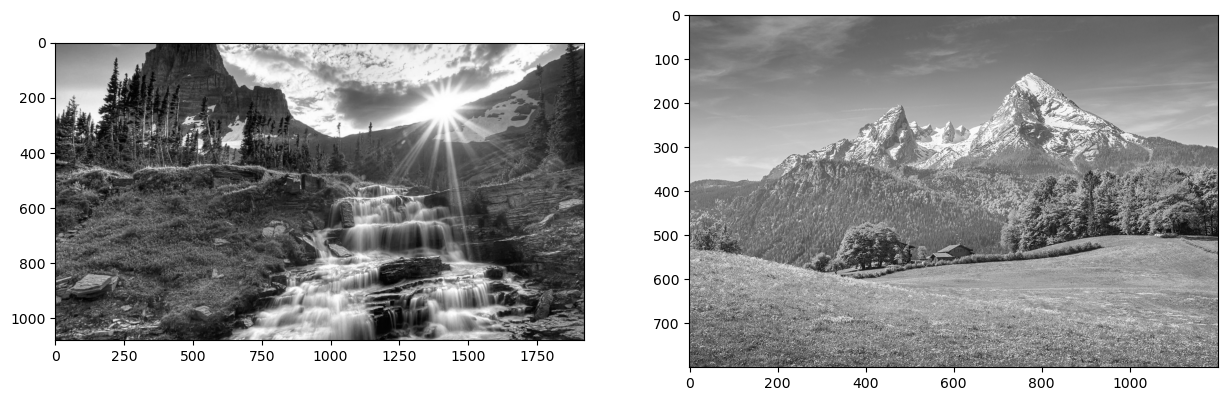
\includegraphics[width=1\textwidth]{output_II_29.png}
\end{center}

\begin{lstlisting}[language=Python]
image_01.shape
\end{lstlisting}

\begin{lstlisting}[language=Python]
(800, 1200)
\end{lstlisting}

\begin{lstlisting}[language=Python]
image_02.shape
\end{lstlisting}

\begin{lstlisting}[language=Python]
(1080, 1920)
\end{lstlisting}

\begin{lstlisting}[language=Python]
print("Euclidean distance between images:", measure_euclid_dist(image_01, image_02))
\end{lstlisting}

\begin{lstlisting}[language=Python]
Euclidean distance between images: 82911.17
\end{lstlisting}


\vspace{1em}
\textbf{AI-Generated}



\begin{lstlisting}[language=Python]
from PIL import Image
import numpy as np
from numpy.linalg import norm

def load_and_preprocess_image(path, size=(256, 256), grayscale=True):
    """
    Load and preprocess the image.
    Resize and optionally convert to grayscale.
    """
    img = Image.open(path)
    if grayscale:
        img = img.convert("L")  # Convert to grayscale
    img = img.resize(size)     # Resize to uniform size
    return np.array(img)

def euclidean_distance(img1_array, img2_array):
    """
    Compute the Euclidean distance between two image arrays.
    """
    if img1_array.shape != img2_array.shape:
        raise ValueError("Images must be of the same shape")

    # Flatten the images into 1D vectors
    vec1 = img1_array.flatten()
    vec2 = img2_array.flatten()

    # Compute Euclidean distance
    distance = norm(vec1 - vec2)
    return distance

# Example usage
if __name__ == "__main__":
    img_path1 = "../images/scenery_01.jpg"
    img_path2 = "../images/scenery_02.jpg"

    try:
        img1 = load_and_preprocess_image(img_path1)
        img2 = load_and_preprocess_image(img_path2)
        
        distance = euclidean_distance(img1, img2)
        print(f"Euclidean distance between the images: {distance:.2f}")
    except Exception as e:
        print("Error:", e)

\end{lstlisting}

\vspace{1em}

\textbf{Comments on comparisons}

\begin{itemize}
    \item The code I have written uses GPU acceleration with CuPy and opencv for image processing and distance computation whereas the AI provided code uses CPU-based libraries like NumPy and PIL.
    \item The AI provided code included explicit image resizing and grayscale conversion for preprocessing.
\end{itemize}
\vspace{1em}

\textbf{Results}

\begin{lstlisting}[language=Python]
Euclidean distance between the images: 33177.28
\end{lstlisting}

\textbf{Verified By}


\newpage

\section*{Cycle II}
\begin{center}
\textbf{Experiment 5}
\label{exp5}
\end{center}

\vspace{1em}

\raggedright{
  \textbf{Problem}\par
  \noindent
  Apply Principal Component Analysis (PCA) and Linear Discriminant Analysis (LDA) on MNIST dataset. Compare the performance of PCA vs. LDA for classifying handwritten digits (MNIST dataset).\par
}


\vspace{1em}

\textbf{Aim and Objectives}

To understand the differences between PCA and LDA in terms of dimensionality reduction and classification performance on the MNIST dataset, and to implement both techniques to compare their effectiveness in classifying handwritten digits.
\vspace{1em}

\textbf{Program Code}

\begin{lstlisting}[language=Python]
import pandas as pd
from sklearn.decomposition import PCA
from sklearn.discriminant_analysis import LinearDiscriminantAnalysis
from sklearn.metrics import classification_report, confusion_matrix
from sklearn.neighbors import KNeighborsClassifier
import pandas as pd
from sklearn.preprocessing import StandardScaler
import matplotlib.pyplot as plt
import seaborn as sns
import numpy as np
\end{lstlisting}

\begin{lstlisting}[language=Python]
Loading the MNIST train and test csv
\end{lstlisting}

\begin{lstlisting}[language=Python]
image_01 = cv2.imread("../images/scenery_01.jpg", cv2.IMREAD_GRAYSCALE)
image_02 = cv2.imread("../images/scenery_02.jpg", cv2.IMREAD_GRAYSCALE)

plt.subplots(1, 2, figsize=(15, 10))
plt.imshow(image_01, cmap='gray')
plt.subplot(1, 2, 1)
plt.imshow(image_02, cmap='gray')
plt.show()
\end{lstlisting}

\begin{lstlisting}[language=Python]
train_set = pd.read_csv("../datasets/mnist_train.csv")
test_set = pd.read_csv("../datasets/mnist_test.csv")
\end{lstlisting}

\begin{lstlisting}[language=Python]
train_set["label"].unique()
\end{lstlisting}

\begin{lstlisting}[language=Python]
array([5, 0, 4, 1, 9, 2, 3, 6, 7, 8])
\end{lstlisting}

\begin{lstlisting}[language=Python]
train_set
\end{lstlisting}

\begin{center}
  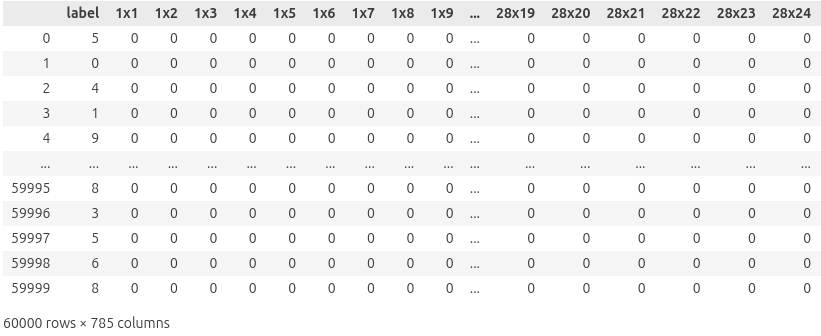
\includegraphics[width=1\textwidth]{output_II_30.png}
\end{center}

\begin{lstlisting}[language=Python]
test_set
\end{lstlisting}

\begin{center}
  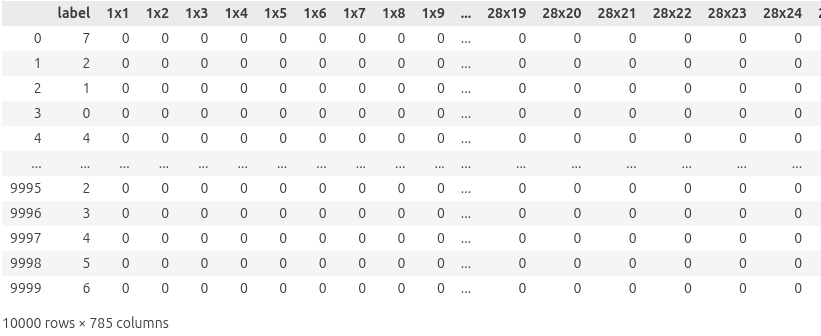
\includegraphics[width=1\textwidth]{output_II_31.png}
\end{center}

\begin{lstlisting}[language=Python]
train_set.describe()
\end{lstlisting}

\begin{center}
  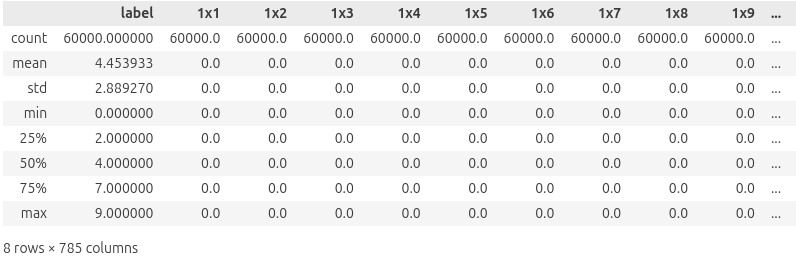
\includegraphics[width=1\textwidth]{output_II_32.png}
\end{center}

\begin{lstlisting}[language=Python]
test_set.describe()
\end{lstlisting}

\begin{center}
  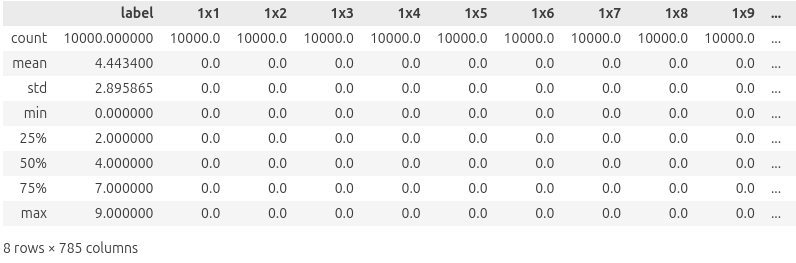
\includegraphics[width=1\textwidth]{output_II_33.png}
\end{center}

\begin{lstlisting}[language=Python]
Euclidean distance between images: 82911.17
\end{lstlisting}

\begin{lstlisting}[language=Python]
The MNIST dataset contains 10 classes(0 to 9) of handwritten digits each of size 28x28
\end{lstlisting}

\begin{lstlisting}[language=Python]
plt.subplots(1, 10, figsize=(20, 17))

for i in range(10):
    plt.subplot(1, 10, i + 1)
    # plt.imshow(train_set[train_set["label"] == i].values[0][1:].reshape(28, 28), cmap="gray")
    image = train_set[train_set["label"] == i].to_numpy()[0][1:].reshape(28, 28)
    plt.imshow(image, cmap="gray")
    plt.axis("off")
    plt.title(i)
plt.show()

\end{lstlisting}

\begin{center}
  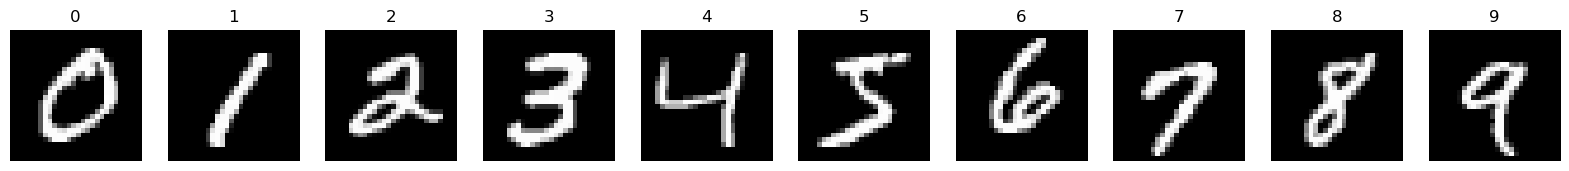
\includegraphics[width=1\textwidth]{output_II_03.png}
\end{center}

\begin{lstlisting}[language=Python]
train_set_copy = train_set.copy()
train_set_copy = train_set_copy.drop(columns=["label"])
\end{lstlisting}

\begin{lstlisting}[language=Python]
test_set_copy = test_set.copy()
test_set_copy = test_set_copy.drop(columns=["label"])
\end{lstlisting}

\begin{lstlisting}[language=Python]
Scaling the values of both the sets
\end{lstlisting}

\begin{lstlisting}[language=Python]
std_scaler = StandardScaler()
train_set_copy = std_scaler.fit_transform(train_set_copy)
test_set_copy = std_scaler.transform(test_set_copy)
\end{lstlisting}

\begin{lstlisting}[language=Python]
Applying PCA on the dataset
\end{lstlisting}

\begin{lstlisting}[language=Python]
pca = PCA(n_components=50)
train_set_pca = pca.fit_transform(train_set_copy)
pca.explained_variance_ratio_
\end{lstlisting}

\begin{lstlisting}[language=Python]
array([0.09704664, 0.07095924, 0.06169089, 0.05389419, 0.04868797,
       0.04312231, 0.0327193 , 0.02883895, 0.02762029, 0.02357001,
       0.0210919 , 0.02022991, 0.01715818, 0.01692111, 0.01578641,
       0.01482953, 0.01324561, 0.01276897, 0.01187263, 0.01152684,
       0.01066166, 0.01006713, 0.00953573, 0.00912544, 0.00883405,
       0.00839319, 0.00812579, 0.00786366, 0.00744733, 0.00690859,
       0.00658094, 0.00648148, 0.00602615, 0.00586582, 0.00570021,
       0.00543628, 0.00505786, 0.00487859, 0.00481429, 0.00472266,
       0.00456747, 0.00444836, 0.00418501, 0.00398215, 0.00384975,
       0.00375103, 0.00362009, 0.00351591, 0.00340058, 0.00321874])
\end{lstlisting}

\begin{lstlisting}[language=Python]
test_set_pca = pca.fit_transform(test_set_copy)
\end{lstlisting}

\begin{lstlisting}[language=Python]
Applying LDA on the dataset
\end{lstlisting}

\begin{lstlisting}[language=Python]
lda = LinearDiscriminantAnalysis(n_components=9)
train_set_lda = lda.fit_transform(train_set_copy, train_set["label"])
lda.explained_variance_ratio_
\end{lstlisting}

\begin{lstlisting}[language=Python]
array([0.2392286 , 0.20180995, 0.17849695, 0.10652571, 0.09406712,
       0.06906025, 0.04973746, 0.03429077, 0.0267832 ])
\end{lstlisting}

\begin{lstlisting}[language=Python]
test_set_lda = lda.fit_transform(test_set_copy, test_set["label"])
\end{lstlisting}

\begin{lstlisting}[language=Python]
Training two KNN models on the two train sets
\end{lstlisting}

\begin{lstlisting}[language=Python]
knn_01 = KNeighborsClassifier(n_neighbors=5)

knn_02 = KNeighborsClassifier(n_neighbors=5)
\end{lstlisting}

\begin{lstlisting}[language=Python]
knn_01.fit(train_set_pca, train_set["label"])
\end{lstlisting}

\begin{center}
  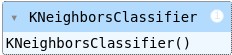
\includegraphics[width=0.25\textwidth]{output_II_34.png}
\end{center}

\begin{lstlisting}[language=Python]
knn_02.fit(train_set_lda, train_set["label"])
\end{lstlisting}

\begin{center}
  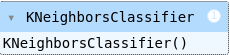
\includegraphics[width=0.25\textwidth]{output_II_35.png}
\end{center}

\begin{lstlisting}[language=Python]
Evaluating the performance of the two SVMs
\end{lstlisting}

\begin{lstlisting}[language=Python]
pred_01 = knn_01.predict(test_set_pca)
pred_02 = knn_02.predict(test_set_lda)
\end{lstlisting}

\begin{lstlisting}[language=Python]
print("PCA Classification Report")
print(classification_report(test_set["label"], pred_01))
\end{lstlisting}

\begin{lstlisting}[language=Python]
PCA Classification Report
              precision    recall  f1-score   support

           0       0.80      0.80      0.80       980
           1       0.80      0.68      0.74      1135
           2       0.52      0.53      0.52      1032
           3       0.67      0.76      0.71      1010
           4       0.66      0.68      0.67       982
           5       0.67      0.62      0.64       892
           6       0.43      0.33      0.37       958
           7       0.57      0.58      0.57      1028
           8       0.59      0.67      0.63       974
           9       0.61      0.69      0.65      1009

    accuracy                           0.64     10000
   macro avg       0.63      0.63      0.63     10000
weighted avg       0.64      0.64      0.63     10000
\end{lstlisting}

\begin{lstlisting}[language=Python]
confusion_matrix_01 = confusion_matrix(test_set["label"], pred_01)
sns.heatmap(confusion_matrix_01, annot=True, fmt="d", cmap="Blues")
\end{lstlisting}

\begin{center}
  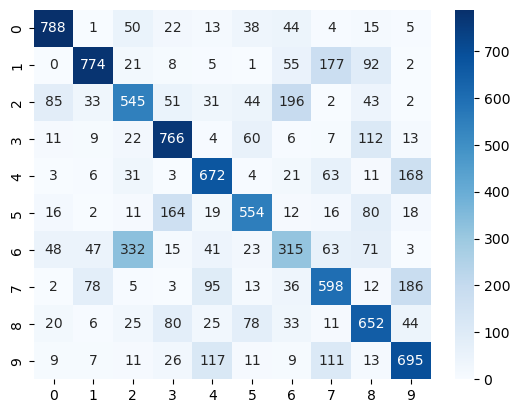
\includegraphics[width=0.7\textwidth]{output_II_36.png}
\end{center}

\begin{lstlisting}[language=Python]
print("LDA Classification Report")
print(classification_report(test_set["label"], pred_02))
\end{lstlisting}

\begin{lstlisting}[language=Python]
LDA Classification Report
              precision    recall  f1-score   support

           0       0.96      0.96      0.96       980
           1       0.93      0.88      0.91      1135
           2       0.91      0.91      0.91      1032
           3       0.89      0.90      0.90      1010
           4       0.89      0.93      0.91       982
           5       0.89      0.85      0.87       892
           6       0.96      0.96      0.96       958
           7       0.73      0.95      0.82      1028
           8       0.87      0.86      0.86       974
           9       0.91      0.68      0.78      1009

    accuracy                           0.89     10000
   macro avg       0.89      0.89      0.89     10000
weighted avg       0.89      0.89      0.89     10000
\end{lstlisting}

\begin{lstlisting}[language=Python]
confusion_matrix_02 = confusion_matrix(test_set["label"], pred_02)
sns.heatmap(confusion_matrix_02, annot=True, fmt="d", cmap="Blues")
\end{lstlisting}

\begin{center}
  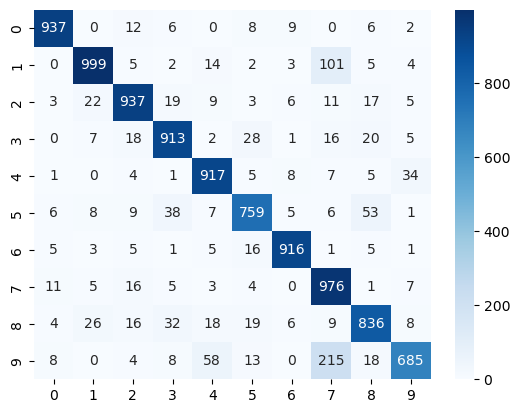
\includegraphics[width=0.7\textwidth]{output_II_37.png}
\end{center}

\vspace{1em}
\textbf{AI-Generated}

\begin{lstlisting}[language=Python]
import numpy as np
import matplotlib.pyplot as plt
from sklearn.datasets import fetch_openml
from sklearn.decomposition import PCA
from sklearn.discriminant_analysis import LinearDiscriminantAnalysis as LDA
from sklearn.model_selection import train_test_split
from sklearn.neighbors import KNeighborsClassifier
from sklearn.metrics import accuracy_score, classification_report

# Load MNIST dataset
print("Loading MNIST dataset...")
X, y = fetch_openml('mnist_784', version=1, return_X_y=True, as_frame=False)
y = y.astype(int)

# Train-test split
print("Splitting dataset...")
X_train, X_test, y_train, y_test = train_test_split(X, y, test_size=0.2, random_state=42)

# Apply PCA (to 50 components)
print("Applying PCA...")
pca = PCA(n_components=50)
X_train_pca = pca.fit_transform(X_train)
X_test_pca = pca.transform(X_test)

# Apply LDA (for classification - full 9 components)
print("Applying LDA for classification...")
lda_full = LDA(n_components=9)
X_train_lda = lda_full.fit_transform(X_train, y_train)
X_test_lda = lda_full.transform(X_test)

# Train KNN on PCA
print("Training KNN on PCA...")
knn_pca = KNeighborsClassifier(n_neighbors=3)
knn_pca.fit(X_train_pca, y_train)
y_pred_pca = knn_pca.predict(X_test_pca)
acc_pca = accuracy_score(y_test, y_pred_pca)

# Train KNN on LDA
print("Training KNN on LDA...")
knn_lda = KNeighborsClassifier(n_neighbors=3)
knn_lda.fit(X_train_lda, y_train)
y_pred_lda = knn_lda.predict(X_test_lda)
acc_lda = accuracy_score(y_test, y_pred_lda)

# Print accuracy
print("\n--- Results ---")
print(f"PCA Accuracy: {acc_pca:.4f}")
print(f"LDA Accuracy: {acc_lda:.4f}")

# Classification Reports
print("\nClassification Report (PCA):")
print(classification_report(y_test, y_pred_pca))
print("\nClassification Report (LDA):")
print(classification_report(y_test, y_pred_lda))

# PCA Explained Variance Plot
plt.figure(figsize=(8, 4))
plt.plot(np.cumsum(pca.explained_variance_ratio_[:100]), marker='o')
plt.title("PCA - Cumulative Explained Variance")
plt.xlabel("Number of Components")
plt.ylabel("Cumulative Variance Explained")
plt.grid(True)
plt.tight_layout()
plt.show()

# LDA Visualization (2D)
print("Visualizing LDA in 2D...")
lda_2d = LDA(n_components=2)
X_lda_2d = lda_2d.fit_transform(X_train, y_train)

plt.figure(figsize=(10, 8))
scatter = plt.scatter(X_lda_2d[:, 0], X_lda_2d[:, 1], c=y_train, cmap='tab10', alpha=0.7, s=10)
plt.title("LDA 2D Visualization of MNIST Training Set")
plt.xlabel("LDA Component 1")
plt.ylabel("LDA Component 2")
plt.legend(*scatter.legend_elements(), title="Digits", loc="best")
plt.grid(True)
plt.tight_layout()
plt.show()
\end{lstlisting}

\textbf{Comments on comparisons}

\begin{itemize}
    \item The AI generated code has performed PCA and LDA on the MNIST dataset, fetched using the built-in fetch\_openml function from scikit-learn, while the code I have written uses a CSV file to load the dataset.
    \item Both codes apply PCA to reduce the dataset to 50 components and LDA to reduce the dataset to 9 components, but the AI code uses KNN with 3 neighbors for classification while my code uses KNN with 5 neighbors.
    \item The AI code includes a visualization of the cumulative explained variance for PCA and a 2D visualization of LDA components, while my code focuses on classification performance and confusion matrices.
\end{itemize}

\textbf{Results}

\begin{lstlisting}[language=Python]
Loading MNIST dataset...
Splitting dataset...
Applying PCA...
Applying LDA for classification...
Training KNN on PCA...
Training KNN on LDA...

--- Results ---
PCA Accuracy: 0.9772
LDA Accuracy: 0.9109

Classification Report (PCA):
              precision    recall  f1-score   support

           0       0.98      1.00      0.99      1343
           1       0.98      0.99      0.99      1600
           2       0.97      0.97      0.97      1380
           3       0.97      0.96      0.97      1433
           4       0.97      0.98      0.98      1295
           5       0.98      0.97      0.97      1273
           6       0.99      0.99      0.99      1396
           7       0.98      0.98      0.98      1503
           8       0.99      0.96      0.97      1357
           9       0.97      0.97      0.97      1420

    accuracy                           0.98     14000
   macro avg       0.98      0.98      0.98     14000
weighted avg       0.98      0.98      0.98     14000


Classification Report (LDA):
              precision    recall  f1-score   support

           0       0.94      0.97      0.96      1343
           1       0.92      0.98      0.95      1600
           2       0.89      0.91      0.90      1380
           3       0.89      0.87      0.88      1433
           4       0.89      0.92      0.91      1295
           5       0.87      0.87      0.87      1273
           6       0.96      0.95      0.95      1396
           7       0.95      0.92      0.93      1503
           8       0.89      0.82      0.85      1357
           9       0.90      0.89      0.90      1420

    accuracy                           0.91     14000
   macro avg       0.91      0.91      0.91     14000
weighted avg       0.91      0.91      0.91     14000
\end{lstlisting}

\begin{center}
  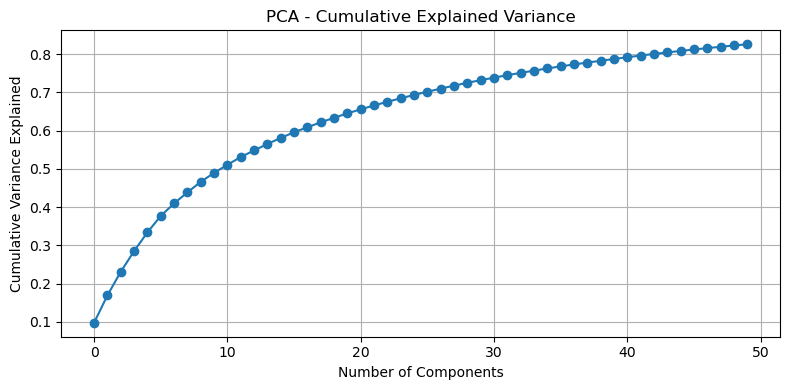
\includegraphics[width=0.6\textwidth]{output_II_38.png}
\end{center}

\begin{lstlisting}[language=Python]
  Visualizing LDA in 2D...
\end{lstlisting}

\begin{center}
  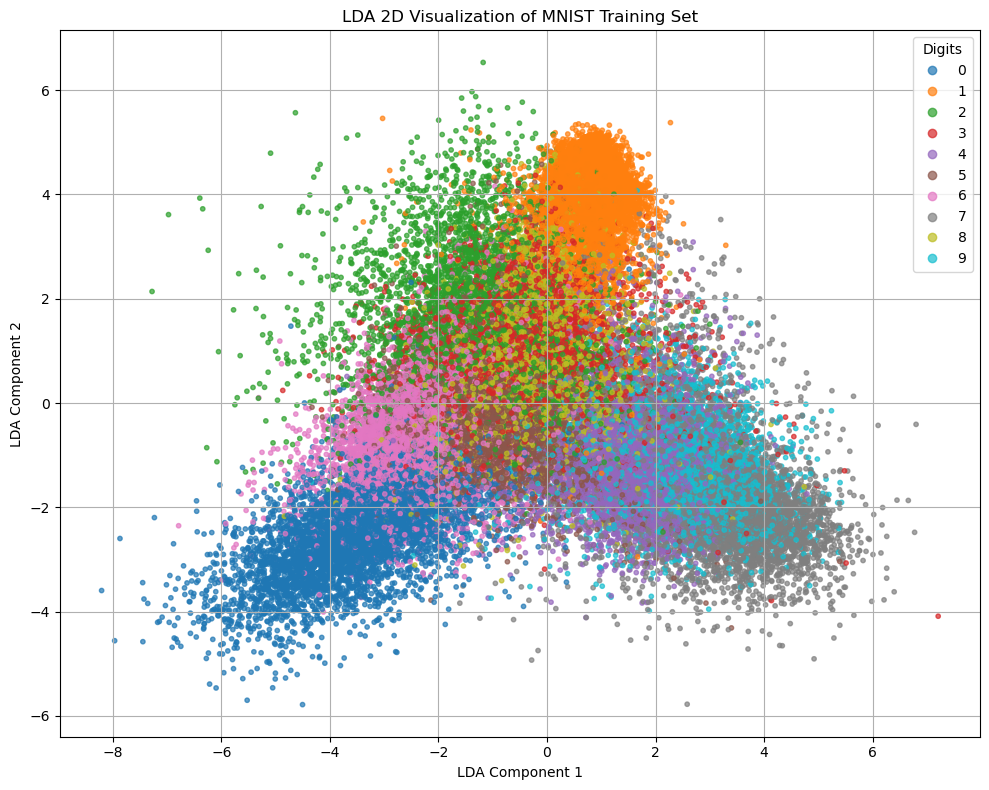
\includegraphics[width=0.6\textwidth]{output_II_39.png}
\end{center}

\textbf{Verified By}


\newpage

\section*{Cycle II}
\begin{center}
\textbf{Experiment 6}
\label{exp6}
\end{center}

\vspace{1em}

\raggedright{
  \textbf{Problem}\par
  \noindent
  Load an image dataset (eg: Iris dataset). Compute the following distances between sample points.
  \begin{itemize}
    \item Hamming Distance
    \item Euclidean Distance
    \item Manhattan (City Block) Distance
  \end{itemize}
}


\vspace{1em}

\textbf{Aim and Objectives}

To understand and implement different distance metrics (Hamming, Euclidean, and Manhattan) on a dataset, specifically the Iris dataset, to analyze the relationships between sample points.
\vspace{1em}

\textbf{Program Code}

\begin{lstlisting}[language=Python]
import cv2
import numpy as np
import matplotlib.pyplot as plt
import os
from scipy.spatial.distance import euclidean, hamming, cityblock

\end{lstlisting}

\begin{lstlisting}[language=Python]
setosa = os.listdir("../datasets/iris/iris-setosa/")
versicolor = os.listdir("../datasets/iris/iris-versicolour/")
virginica = os.listdir("../datasets/iris/iris-virginica/")
\end{lstlisting}

\begin{lstlisting}[language=Python]
x = np.random.randint(0, len(setosa), 1)
image = cv2.imread("../datasets/iris/iris-setosa/" + setosa[x[0]], cv2.IMREAD_GRAYSCALE)

y = np.random.randint(0, len(versicolor), 1)
image2 = cv2.imread("../datasets/iris/iris-versicolour/" + versicolor[y[0]], cv2.IMREAD_GRAYSCALE)

z = np.random.randint(0, len(virginica), 1)
image3 = cv2.imread("../datasets/iris/iris-virginica/" + virginica[z[0]], cv2.IMREAD_GRAYSCALE)

plt.figure(figsize=(10, 10))
plt.subplot(1,3,1)
plt.imshow(image, cmap='gray')
plt.title("Iris Setosa")
plt.axis('off')
plt.subplot(1,3,2)
plt.imshow(image2, cmap='gray')
plt.title("Iris Versicolor")
plt.axis('off')
plt.subplot(1,3,3)
plt.imshow(image3, cmap='gray')
plt.title("Iris Virginica")
plt.axis('off')
plt.tight_layout()
plt.show()
\end{lstlisting}

\begin{center}
  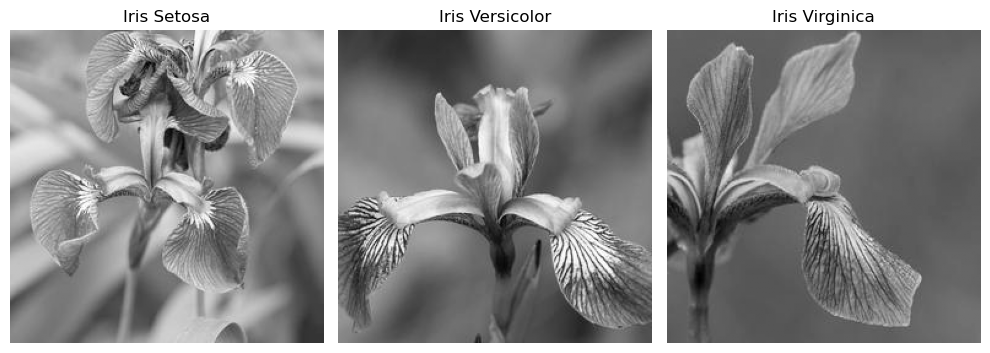
\includegraphics[width=1\textwidth]{output_II_40.png}
\end{center}

\begin{lstlisting}[language=Python]
Calculating the hamming distance between two images
\end{lstlisting}

\begin{lstlisting}[language=Python]
image_bin =  cv2.adaptiveThreshold(image, 255, cv2.ADAPTIVE_THRESH_GAUSSIAN_C, cv2.THRESH_BINARY, 11, 2)
image2_bin =  cv2.adaptiveThreshold(image2, 255, cv2.ADAPTIVE_THRESH_GAUSSIAN_C, cv2.THRESH_BINARY, 11, 2)

image3_bin = cv2.adaptiveThreshold(image3, 255, cv2.ADAPTIVE_THRESH_GAUSSIAN_C, cv2.THRESH_BINARY, 11, 2)
\end{lstlisting}

\begin{lstlisting}[language=Python]
print("Hamming Distance between Setosa and Versicolor: ", ham_1)
print("Hamming Distance between Setosa and Virginica: ", ham_2)
print("Hamming Distance between Versicolor and Virginica: ", ham_3)

Hamming Distance between Setosa and Versicolor:  0.385467529296875
Hamming Distance between Setosa and Virginica:  0.374298095703125
Hamming Distance between Versicolor and Virginica:  0.307220458984375
\end{lstlisting}

\begin{lstlisting}[language=Python]
euc_1 = euclidean(image_bin.flatten(), image2_bin.flatten())
euc_2 = euclidean(image_bin.flatten(), image3_bin.flatten())
euc_3 = euclidean(image2_bin.flatten(), image3_bin.flatten())

print("Euclidean Distance between Setosa and Versicolor: ", euc_1)
print("Euclidean Distance between Setosa and Virginica: ", euc_2)
print("Euclidean Distance between Versicolor and Virginica: ", euc_3)
\end{lstlisting}

\begin{lstlisting}[language=Python]
Euclidean Distance between Setosa and Versicolor:  24284.314237795556
Euclidean Distance between Setosa and Virginica:  23709.85048455599
Euclidean Distance between Versicolor and Virginica:  25511.670858648205
\end{lstlisting}

\begin{lstlisting}[language=Python]
cityblock_1 = cityblock(image_bin.flatten(), image2_bin.flatten())
cityblock_2 = cityblock(image_bin.flatten(), image3_bin.flatten())
cityblock_3 = cityblock(image2_bin.flatten(), image3_bin.flatten())

print("Cityblock Distance between Setosa and Versicolor: ", cityblock_1)
print("Cityblock Distance between Setosa and Virginica: ", cityblock_2)
print("Cityblock Distance between Versicolor and Virginica: ", cityblock_3)
\end{lstlisting}

\begin{lstlisting}[language=Python]
Cityblock Distance between Setosa and Versicolor:  2328788
Cityblock Distance between Setosa and Virginica:  2220360
Cityblock Distance between Versicolor and Virginica:  2562420
\end{lstlisting}

\vspace{1em}
\textbf{AI-Generated}

\begin{lstlisting}[language=Python]
import numpy as np
import matplotlib.pyplot as plt
from sklearn.datasets import load_digits
from scipy.spatial.distance import euclidean, cityblock, hamming
from itertools import combinations

# Load sample image dataset (use this or replace with your own image loader)
digits = load_digits()
images = digits.images
labels = digits.target

# Flatten images into 1D vectors
flattened_images = images.reshape((images.shape[0], -1))

# Select a few samples for demonstration
sample_indices = [0, 1, 2]  # You can change these
samples = flattened_images[sample_indices]
sample_labels = labels[sample_indices]

# Compute and display distances between pairs
print("Distance Metrics Between Sample Images:\n")

for (i, a), (j, b) in combinations(enumerate(samples), 2):
    eu_dist = euclidean(a, b)
    man_dist = cityblock(a, b)
    ham_dist = hamming(a > 0, b > 0)  # Convert to binary for Hamming
    
    print(f"Image {sample_labels[i]} vs Image {sample_labels[j]}:")
    print(f"  Euclidean Distance : {eu_dist:.4f}")
    print(f"  Manhattan Distance : {man_dist:.4f}")
    print(f"  Hamming Distance   : {ham_dist:.4f}\n")

# Optional: Visualize the sample images
fig, axes = plt.subplots(1, len(sample_indices), figsize=(10, 3))
for ax, idx in zip(axes, sample_indices):
    ax.imshow(images[idx], cmap='gray')
    ax.set_title(f"Label: {labels[idx]}")
    ax.axis("off")
plt.tight_layout()
plt.show()
\end{lstlisting}

\vspace{1em}

\textbf{Comments on comparisons}

\begin{itemize}
    \item The AI-generated code uses the `load\_digits` function from scikit-learn to load a sample image dataset, while my code uses images from the Iris dataset.
    \item The AI code computes distances between pairs of images using Euclidean, Manhattan, and Hamming metrics, similar to my code.
    \item The AI code uses `combinations` from the `itertools` module to compute distances between all pairs of selected samples, while my code computes distances between three specific images from the Iris dataset.
\end{itemize}
\vspace{1em}

\textbf{Results}

\begin{lstlisting}[language=Python]
Distance Metrics Between Sample Images:

Image 0 vs Image 1:
  Euclidean Distance : 59.5567
  Manhattan Distance : 335.0000
  Hamming Distance   : 0.2969

Image 0 vs Image 2:
  Euclidean Distance : 54.1295
  Manhattan Distance : 306.0000
  Hamming Distance   : 0.2969

Image 1 vs Image 2:
  Euclidean Distance : 41.6293
  Manhattan Distance : 205.0000
  Hamming Distance   : 0.1250
\end{lstlisting}

\begin{center}
  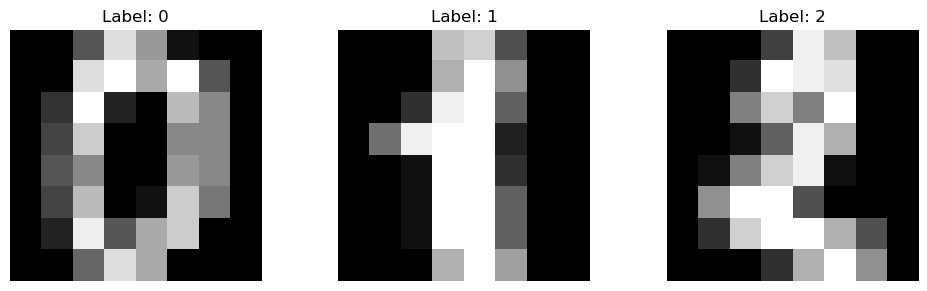
\includegraphics[width=0.7\textwidth]{output_II_41.png}
\end{center}


\textbf{Verified By}

\newpage

\section*{Cycle II}
\begin{center}
\textbf{Experiment 7}
\label{exp7}
\end{center}

\vspace{1em}

\raggedright{
  \textbf{Problem}\par
  \noindent
  Perform union, intersection, and complement operations on two fuzzy sets. Visualize the fuzzy sets and their operations. Implement De Morgans law on Fuzzy sets.
}


\vspace{1em}

\textbf{Aim and Objectives}

To understand and implement fuzzy set operations such as union, intersection, and complement, and to visualize these operations. Additionally, to apply De Morgan's law on fuzzy sets.
\vspace{1em}

\textbf{Program Code}

\begin{lstlisting}[language=Python]
import matplotlib.pyplot as plt
import random
import numpy as np
import skfuzzy as fuzzy
\end{lstlisting}

\begin{lstlisting}[language=Python]
set_a = np.linspace(0.1, 1, 100)
set_b = np.linspace(0, 1, 100)
\end{lstlisting}

\begin{lstlisting}[language=Python]
m_a = fuzzy.membership.trimf(set_a, [0, 0.5, 1])
m_b = fuzzy.membership.trimf(set_b, [0, 0.8, 1])
\end{lstlisting}

\begin{lstlisting}[language=Python]
plt.subplots(1, 2, figsize=(12, 5))
plt.subplot(1, 2, 1)
plt.plot(set_a, m_a, 'r', label='Set A')
plt.title('Membership Function of Set A')
plt.xlabel('Universe of Discourse')
plt.ylabel('Membership Degree')
plt.legend()
plt.grid()
plt.subplot(1, 2, 2)
plt.plot(set_b, m_b, 'b', label='Set B')
plt.title('Membership Function of Set B')
plt.xlabel('Universe of Discourse')
plt.ylabel('Membership Degree')
plt.legend()
plt.grid()
\end{lstlisting}

\begin{center}
  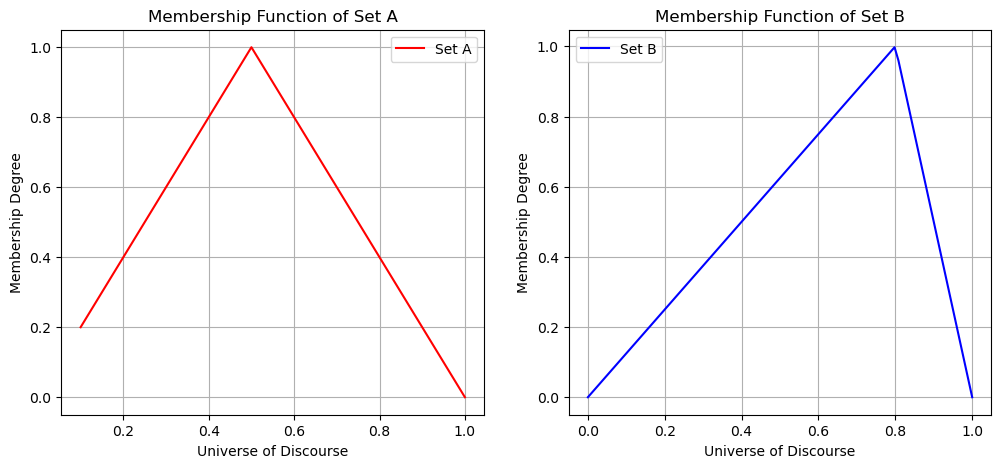
\includegraphics[width=1\textwidth]{output_II_42.png}
\end{center}

\begin{lstlisting}[language=Python]
union_x, union_y = fuzzy.fuzzy_or(set_a, m_a, set_b, m_b)
plt.figure(figsize=(8,5))
plt.plot(union_x, union_y, 'g', label='Union of A and B')
plt.title('Union of Membership functions A and B')
plt.xlabel('Universe of Discourse')
plt.ylabel('Membership Degree')
plt.legend()
plt.grid()
plt.show()
\end{lstlisting}

\begin{center}
  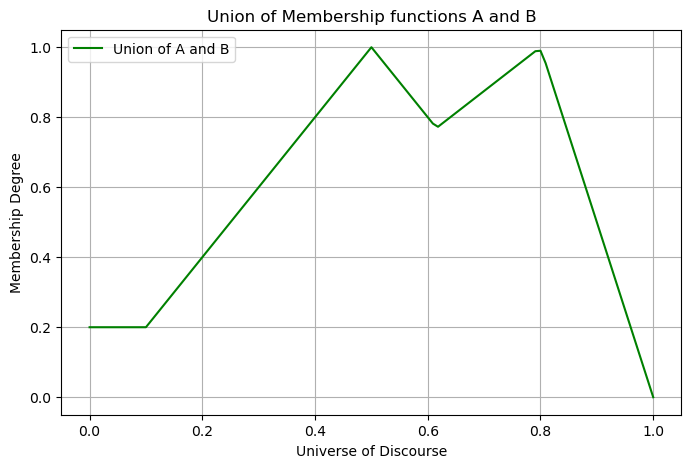
\includegraphics[width=0.65\textwidth]{output_II_43.png}
\end{center}


\begin{lstlisting}[language=Python]
  intersection_x, intersection_y = fuzzy.fuzzy_and(set_a, m_a, set_b, m_b)
  plt.figure(figsize=(8,5))
  plt.plot(intersection_x, intersection_y, 'm', label='Intersection of A and B')
  plt.title('Intersection of Membership functions A and B')
  plt.xlabel('Universe of Discourse')
  plt.ylabel('Membership Degree')
  plt.legend()
  plt.grid()
  plt.show()
\end{lstlisting}

\begin{center}
  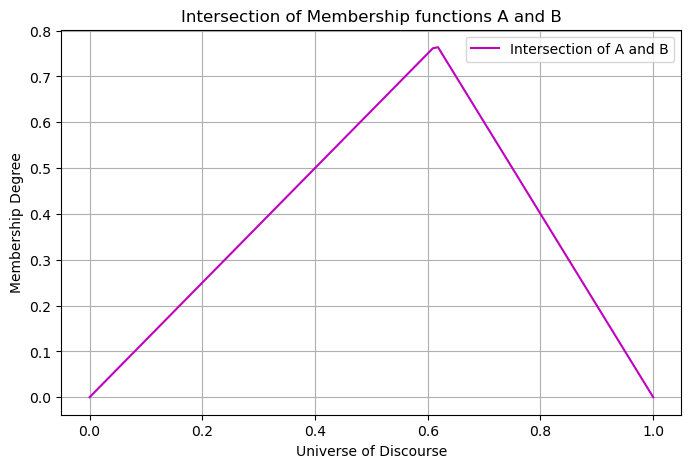
\includegraphics[width=0.65\textwidth]{output_II_44.png}
\end{center}

\begin{lstlisting}[language=Python]
complement_x= fuzzy.fuzzy_not(m_a)
plt.figure(figsize=(8,5))
plt.plot(set_a, complement_x, 'c', label='Complement of A')
plt.title('Complement of Membership function A')
plt.xlabel('Universe of Discourse')
plt.ylabel('Membership Degree')
plt.legend()
plt.grid()
plt.show()
\end{lstlisting}

\begin{center}
  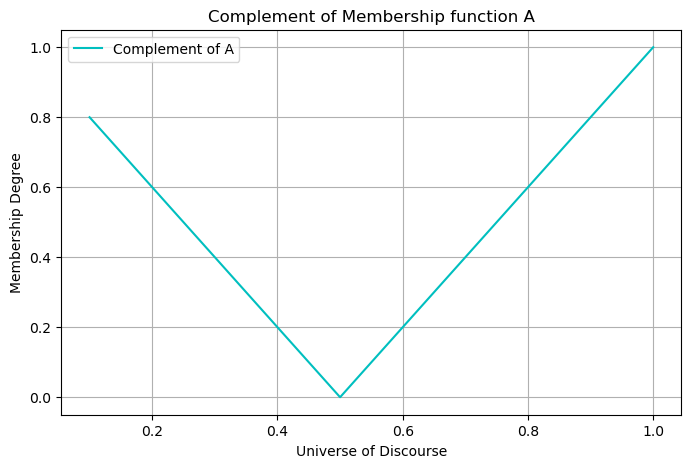
\includegraphics[width=0.65\textwidth]{output_II_45.png}
\end{center}

\begin{lstlisting}[language=Python]
complement_y = fuzzy.fuzzy_not(m_b)
plt.figure(figsize=(8,5))
plt.plot(set_b, complement_y, 'y', label='Complement of B')
plt.title('Complement of Membership function B')
plt.xlabel('Universe of Discourse')
plt.ylabel('Membership Degree')
plt.legend()
plt.grid()
plt.show()
\end{lstlisting}

\begin{center}
  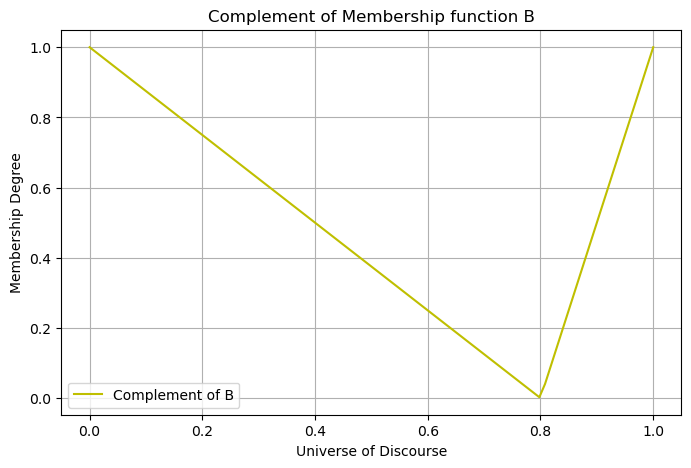
\includegraphics[width=0.65\textwidth]{output_II_46.png}
\end{center}

\begin{lstlisting}[language=Python]
Verifying De Morgan's law using the two fuzzy sets
\end{lstlisting}

\begin{equation*}
\text{De Morgan's first law states that:}
(A \cup B)' = A' \cap B'
\end{equation*}

\begin{lstlisting}[language=Python]
plt.subplots(1, 2, figsize=(12, 5))
plt.subplot(1, 2, 1)
plt.plot(set_a, m_a, 'r', label='Set A')
plt.title('Membership Function of Set A')
plt.xlabel('Universe of Discourse')
plt.ylabel('Membership Degree')
plt.legend()
plt.grid()
plt.subplot(1, 2, 2)
plt.plot(set_b, m_b, 'b', label='Set B')
plt.title('Membership Function of Set B')
plt.xlabel('Universe of Discourse')
plt.ylabel('Membership Degree')
plt.legend()
plt.grid()
\end{lstlisting}

\begin{center}
  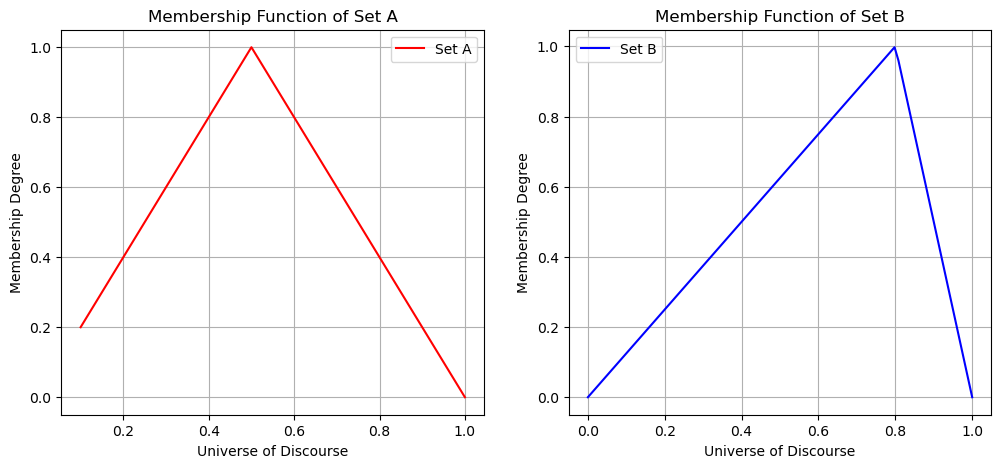
\includegraphics[width=1\textwidth]{output_II_47.png}
\end{center}

\begin{lstlisting}[language=Python]
  union_x, union_y = fuzzy.fuzzy_or(set_a, m_a, set_b, m_b)
  complement_x = fuzzy.fuzzy_not(union_y)
  
  plt.subplots(1, 2, figsize=(12, 5))
  plt.subplot(1, 2, 1)
  plt.plot(union_x, union_y, 'r', label='Union of A and B')
  plt.title('Membership Function of Union of A and B')
  plt.xlabel('Universe of Discourse')
  plt.ylabel('Membership Degree')
  plt.legend()
  plt.grid()
  plt.subplot(1, 2, 2)
  plt.plot(union_x, complement_x, 'b', label='Complement of Union')
  plt.title('Complement of Union of Membership functions A and B')
  plt.xlabel('Universe of Discourse')
  plt.ylabel('Membership Degree')
  plt.legend()
  plt.grid()
\end{lstlisting}

\begin{center}
  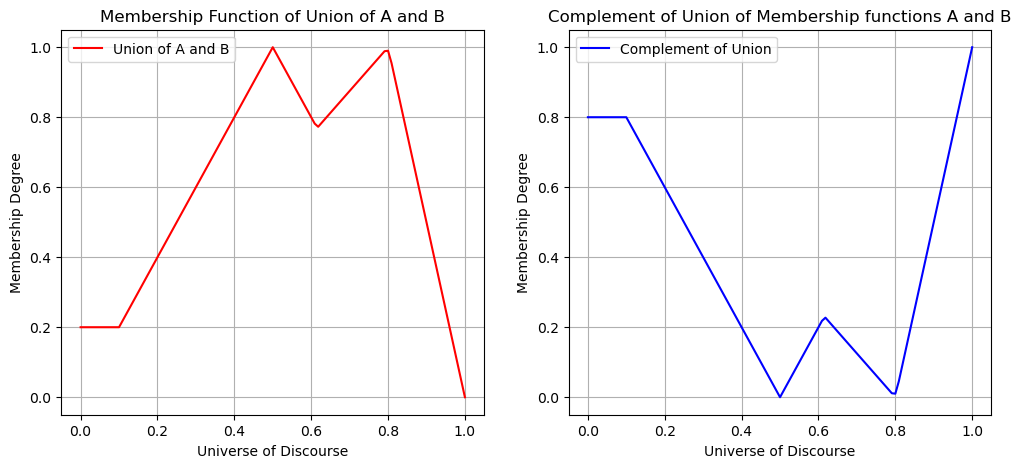
\includegraphics[width=1\textwidth]{output_II_48.png}
\end{center}

\begin{lstlisting}[language=Python]
complement_x = fuzzy.fuzzy_not(m_a)
complement_y = fuzzy.fuzzy_not(m_b)

union_x, union_y = fuzzy.fuzzy_and(set_a, complement_x, set_b, complement_y)

plt.subplots(1, 3, figsize=(18, 5))
plt.subplot(1, 3, 1)
plt.plot(set_a, complement_x, 'r', label='Complement of A')
plt.title('Membership Function of Complement of A')
plt.xlabel('Universe of Discourse')
plt.ylabel('Membership Degree')
plt.legend()
plt.grid()

plt.subplot(1, 3, 2)
plt.plot(set_b, complement_y, 'b', label='Complement of B')
plt.title('Membership Function of Complement of B')
plt.xlabel('Universe of Discourse')
plt.ylabel('Membership Degree')
plt.legend()
plt.grid()

plt.subplot(1, 3, 3)
plt.plot(union_x, union_y, 'g', label='Intersect of Complements of A and B')
plt.title('Intersect of Membership functions of Complements of A and B')
plt.xlabel('Universe of Discourse')
plt.ylabel('Membership Degree')
plt.legend()
plt.grid()
plt.show()
\end{lstlisting}

\begin{center}
  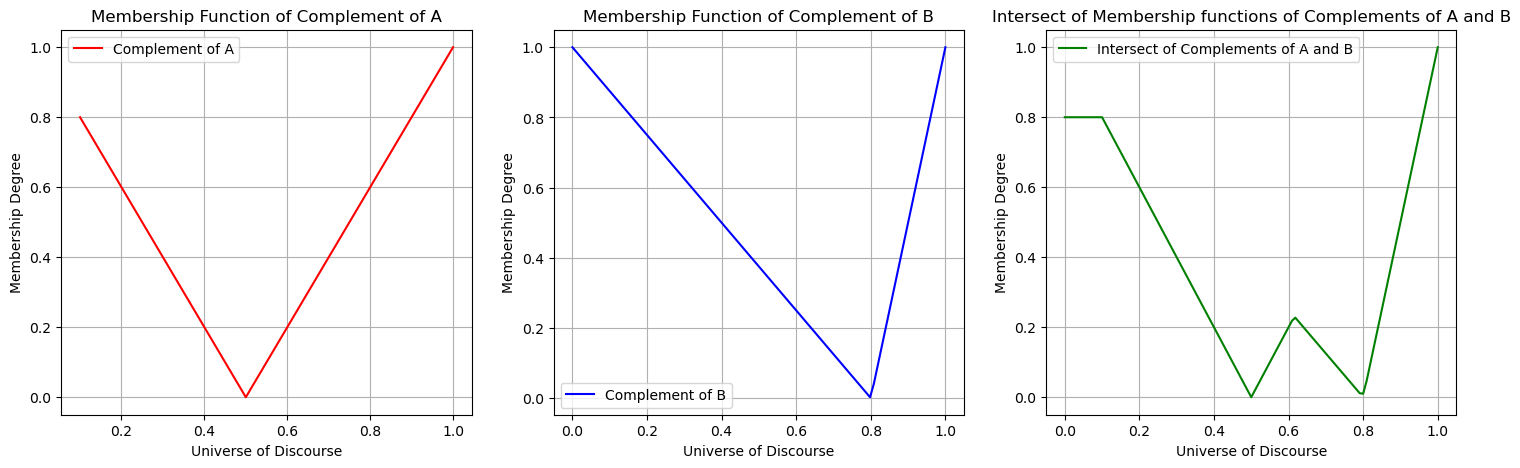
\includegraphics[width=1\textwidth]{output_II_49.png}
\end{center}

\begin{equation*}
\text{De Morgan's second law states that:}
(A \cap B)' = A' \cup B'
\end{equation*}

\begin{lstlisting}[language=Python]
  plt.subplots(1, 2, figsize=(12, 5))
  plt.subplot(1, 2, 1)
  plt.plot(set_a, m_a, 'r', label='Set A')
  plt.title('Membership Function of Set A')
  plt.xlabel('Universe of Discourse')
  plt.ylabel('Membership Degree')
  plt.legend()
  plt.grid()
  plt.subplot(1, 2, 2)
  plt.plot(set_b, m_b, 'b', label='Set B')
  plt.title('Membership Function of Set B')
  plt.xlabel('Universe of Discourse')
  plt.ylabel('Membership Degree')
  plt.legend()
  plt.grid()
\end{lstlisting}

\begin{center}
  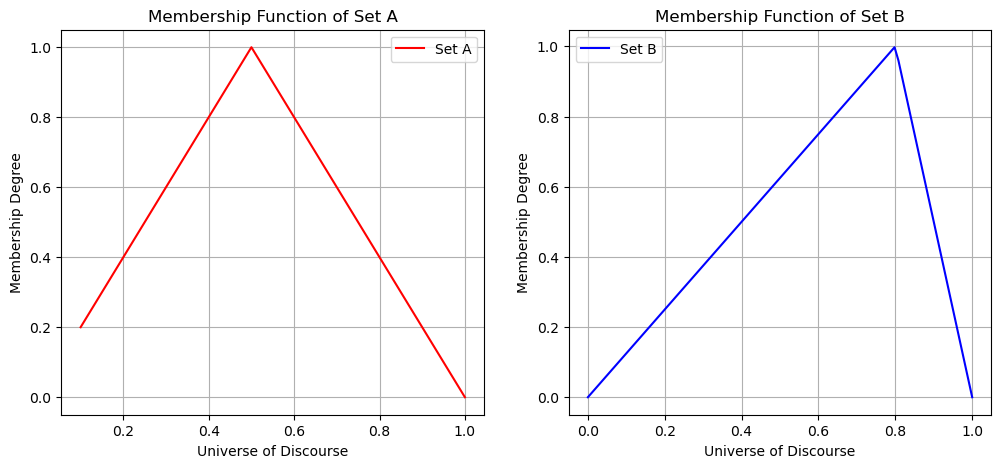
\includegraphics[width=1\textwidth]{output_II_50.png}
\end{center}

\begin{lstlisting}[language=Python]
  intersection_x, intersection_y = fuzzy.fuzzy_and(set_a, m_a, set_b, m_b)
  complement_x = fuzzy.fuzzy_not(intersection_y)
  
  plt.subplots(1, 2, figsize=(12, 5))
  plt.subplot(1, 2, 1)
  plt.plot(intersection_x, intersection_y, 'r', label='Intersection of A and B')
  plt.title('Membership Function of Intersection of A and B')
  plt.xlabel('Universe of Discourse')
  plt.ylabel('Membership Degree')
  plt.legend()
  plt.grid()
  plt.subplot(1, 2, 2)
  plt.plot(union_x, complement_x, 'b', label='Complement of Intersection')
  plt.title('Complement of Intersection of Membership functions A and B')
  plt.xlabel('Universe of Discourse')
  plt.ylabel('Membership Degree')
  plt.legend()
  plt.grid()
\end{lstlisting}

\begin{center}
  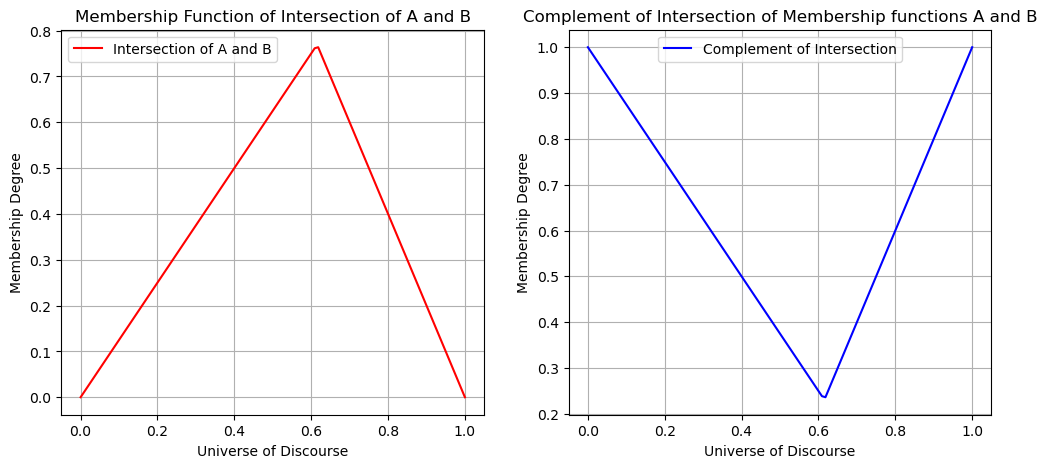
\includegraphics[width=1\textwidth]{output_II_51.png}
\end{center}

\begin{lstlisting}[language=Python]
complement_x = fuzzy.fuzzy_not(m_a)
complement_y = fuzzy.fuzzy_not(m_b)
union_x, union_y = fuzzy.fuzzy_or(set_a, complement_x, set_b, complement_y)
plt.subplots(1, 3, figsize=(18, 5))
plt.subplot(1, 3, 1)
plt.plot(set_a, complement_x, 'r', label='Complement of A')
plt.title('Membership Function of Complement of A')
plt.xlabel('Universe of Discourse')
plt.ylabel('Membership Degree')
plt.legend()
plt.grid()
plt.subplot(1, 3, 2)
plt.plot(set_b, complement_y, 'b', label='Complement of B')
plt.title('Membership Function of Complement of B')
plt.xlabel('Universe of Discourse')
plt.ylabel('Membership Degree')
plt.legend()
plt.grid()
plt.subplot(1, 3, 3)
plt.plot(union_x, union_y, 'g', label='Union of Complements of A and B')
plt.title('Union of Membership functions of Complements of A and B')
plt.xlabel('Universe of Discourse')
plt.ylabel('Membership Degree')
plt.legend()
plt.grid()
plt.show()
\end{lstlisting}

\begin{center}
  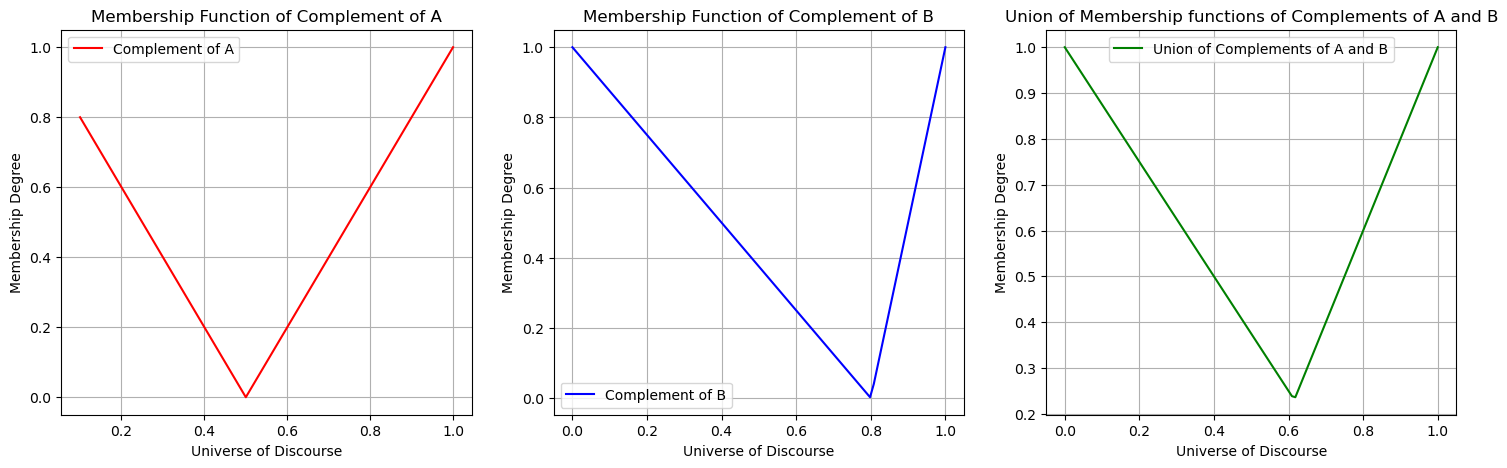
\includegraphics[width=1\textwidth]{output_II_52.png}
\end{center}




\vspace{1em}
\textbf{AI-Generated}

\begin{lstlisting}[language=Python]
import numpy as np
import matplotlib.pyplot as plt

# Define the universe of discourse
x = np.linspace(0, 10, 100)

# Define two fuzzy sets A and B (membership functions)
A = np.maximum(0, 1 - abs(x - 3)/2)  # Triangle centered at 3
B = np.maximum(0, 1 - abs(x - 7)/2)  # Triangle centered at 7

# Fuzzy set operations
union = np.maximum(A, B)
intersection = np.minimum(A, B)
complement_A = 1 - A
complement_B = 1 - B

# De Morgan's Laws
de\_morgan\_1 = 1 - union
de\_morgan\_1\_rhs = np.minimum(complement\_A, complement\_B)

de\_morgan\_2 = 1 - intersection         
de\_morgan\_2\_rhs = np.maximum(complement\_A, complement\_B)

# --- Visualization ---

fig, axs = plt.subplots(3, 2, figsize=(12, 10))
fig.suptitle("Fuzzy Set Operations and De Morgan's Laws", fontsize=16)

# Plot original sets
axs[0, 0].plot(x, A, label='A', color='blue')
axs[0, 0].plot(x, B, label='B', color='red')
axs[0, 0].set_title("Original Fuzzy Sets")
axs[0, 0].legend()
axs[0, 0].grid()

# Union and Intersection
axs[0, 1].plot(x, union, label='A union B', color='purple')
axs[0, 1].plot(x, intersection, label='A intersection B', color='green')
axs[0, 1].set_title("Union and Intersection")
axs[0, 1].legend()
axs[0, 1].grid()

# Complements
axs[1, 0].plot(x, complement_A, label="A'", color='blue', linestyle='--')
axs[1, 0].plot(x, complement_B, label="B'", color='red', linestyle='--')
axs[1, 0].set_title("Complements of A and B")
axs[1, 0].legend()
axs[1, 0].grid()

# De Morgan's Law 1
axs[1, 1].plot(x, de_morgan_1, label="(A union B)'", color='orange')
axs[1, 1].plot(x, de_morgan_1_rhs, label="A' intersection B'", color='green', linestyle='--')
axs[1, 1].set_title("De Morgan's Law 1")
axs[1, 1].legend()
axs[1, 1].grid()

# De Morgan's Law 2
axs[2, 0].plot(x, de_morgan_2, label="(A intersection B)'", color='orange')
axs[2, 0].plot(x, de_morgan_2_rhs, label="A' union B'", color='purple', linestyle='--')
axs[2, 0].set_title("De Morgan's Law 2")
axs[2, 0].legend()
axs[2, 0].grid()

# Hide unused subplot
axs[2, 1].axis('off')

plt.tight_layout(rect=[0, 0, 1, 0.96])
plt.show()
\end{lstlisting}

\vspace{1em}

\textbf{Comments on comparisons}

\begin{itemize}
    \item The AI-generated code uses NumPy and Matplotlib to define and visualize fuzzy sets, while my code uses the skfuzzy library for fuzzy operations.
    \item The AI code visualizes the fuzzy sets and their operations in a single figure with multiple subplots, while my code visualizes each operation in separate figures.
\end{itemize}
\vspace{1em}

\textbf{Results}

\begin{center}
  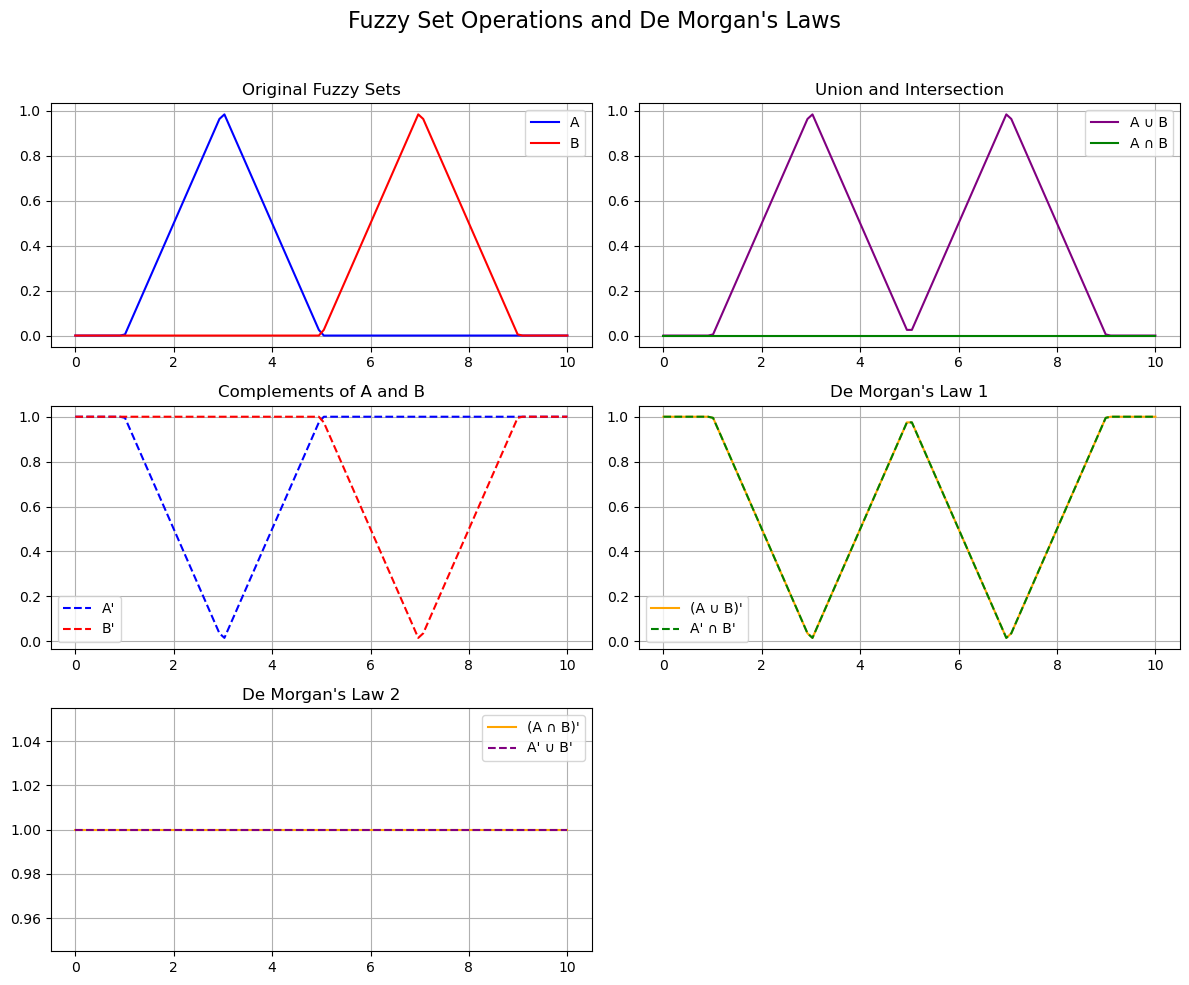
\includegraphics[width=1\textwidth]{output_II_53.png}
\end{center}


\textbf{Verified By}


\newpage

\section*{Cycle II}
\begin{center}
\textbf{Experiment 8}
\label{exp8}
\end{center}

\vspace{1em}

\raggedright{
  \textbf{Problem}\par
  \noindent
  Perform union, intersection, and complement operations on two fuzzy sets. Visualize the fuzzy sets and their operations. Implement De Morgans law on Fuzzy sets.
}


\vspace{1em}

\textbf{Aim and Objectives}

To understand and implement fuzzy set operations such as union, intersection, and complement, and to visualize these operations. Additionally, to apply De Morgan's law on fuzzy sets.
\vspace{1em}

\textbf{Program Code}

\begin{lstlisting}[language=Python]
import matplotlib.pyplot as plt
import random
import numpy as np
import skfuzzy as fuzzy
\end{lstlisting}

\begin{lstlisting}[language=Python]
set_a = np.linspace(0.1, 1, 100)
set_b = np.linspace(0, 1, 100)
\end{lstlisting}

\begin{lstlisting}[language=Python]
m_a = fuzzy.membership.trimf(set_a, [0, 0.5, 1])
m_b = fuzzy.membership.trimf(set_b, [0, 0.8, 1])
\end{lstlisting}

\begin{lstlisting}[language=Python]
plt.subplots(1, 2, figsize=(12, 5))
plt.subplot(1, 2, 1)
plt.plot(set_a, m_a, 'r', label='Set A')
plt.title('Membership Function of Set A')
plt.xlabel('Universe of Discourse')
plt.ylabel('Membership Degree')
plt.legend()
plt.grid()
plt.subplot(1, 2, 2)
plt.plot(set_b, m_b, 'b', label='Set B')
plt.title('Membership Function of Set B')
plt.xlabel('Universe of Discourse')
plt.ylabel('Membership Degree')
plt.legend()
plt.grid()
\end{lstlisting}

\begin{center}
  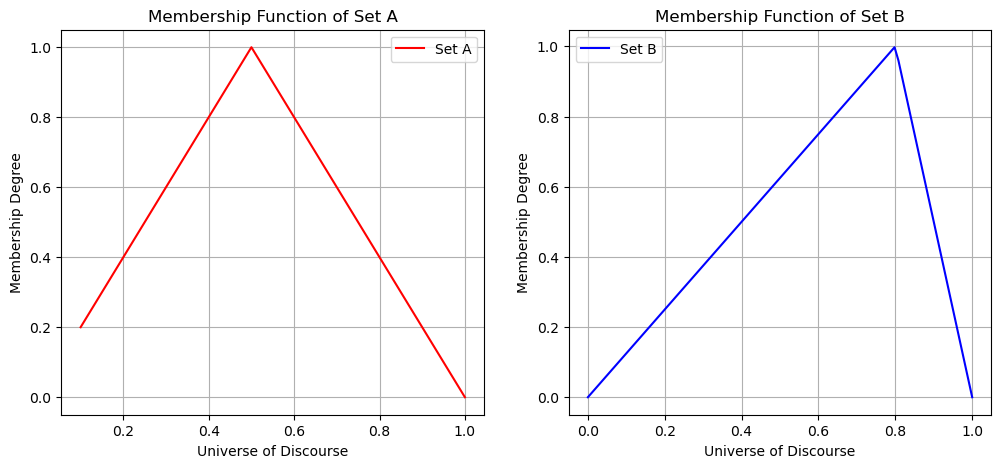
\includegraphics[width=1\textwidth]{output_II_42.png}
\end{center}

\begin{lstlisting}[language=Python]
union_x, union_y = fuzzy.fuzzy_or(set_a, m_a, set_b, m_b)
plt.figure(figsize=(8,5))
plt.plot(union_x, union_y, 'g', label='Union of A and B')
plt.title('Union of Membership functions A and B')
plt.xlabel('Universe of Discourse')
plt.ylabel('Membership Degree')
plt.legend()
plt.grid()
plt.show()
\end{lstlisting}

\begin{center}
  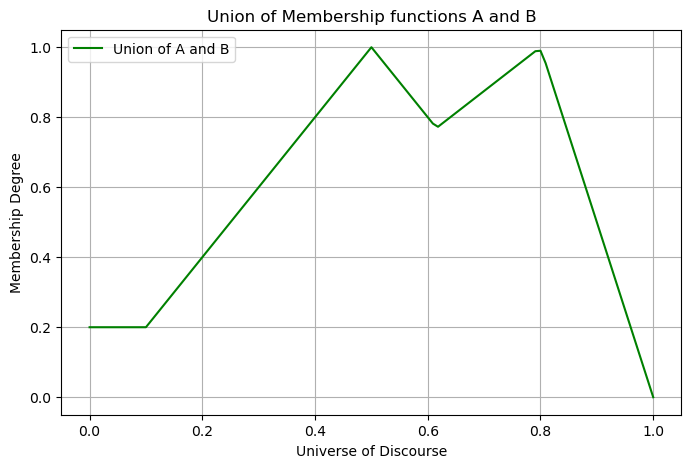
\includegraphics[width=0.65\textwidth]{output_II_43.png}
\end{center}


\begin{lstlisting}[language=Python]
  intersection_x, intersection_y = fuzzy.fuzzy_and(set_a, m_a, set_b, m_b)
  plt.figure(figsize=(8,5))
  plt.plot(intersection_x, intersection_y, 'm', label='Intersection of A and B')
  plt.title('Intersection of Membership functions A and B')
  plt.xlabel('Universe of Discourse')
  plt.ylabel('Membership Degree')
  plt.legend()
  plt.grid()
  plt.show()
\end{lstlisting}

\begin{center}
  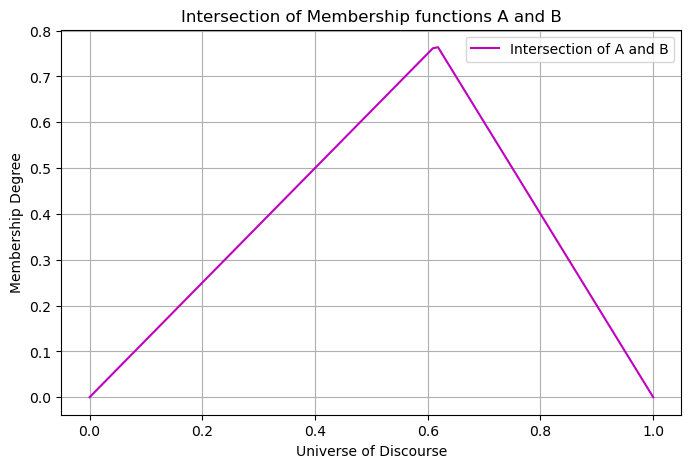
\includegraphics[width=0.65\textwidth]{output_II_44.png}
\end{center}

\begin{lstlisting}[language=Python]
complement_x= fuzzy.fuzzy_not(m_a)
plt.figure(figsize=(8,5))
plt.plot(set_a, complement_x, 'c', label='Complement of A')
plt.title('Complement of Membership function A')
plt.xlabel('Universe of Discourse')
plt.ylabel('Membership Degree')
plt.legend()
plt.grid()
plt.show()
\end{lstlisting}

\begin{center}
  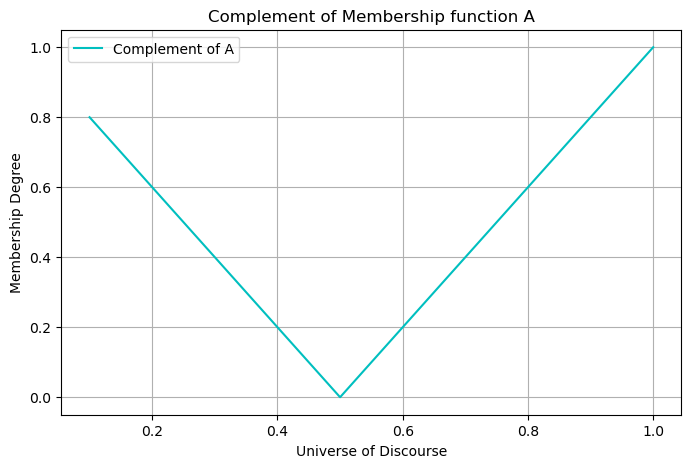
\includegraphics[width=0.65\textwidth]{output_II_45.png}
\end{center}

\begin{lstlisting}[language=Python]
complement_y = fuzzy.fuzzy_not(m_b)
plt.figure(figsize=(8,5))
plt.plot(set_b, complement_y, 'y', label='Complement of B')
plt.title('Complement of Membership function B')
plt.xlabel('Universe of Discourse')
plt.ylabel('Membership Degree')
plt.legend()
plt.grid()
plt.show()
\end{lstlisting}

\begin{center}
  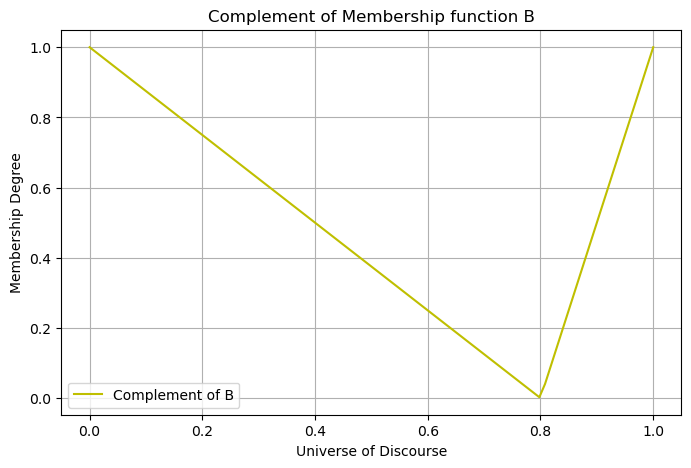
\includegraphics[width=0.65\textwidth]{output_II_46.png}
\end{center}

\begin{lstlisting}[language=Python]
Verifying De Morgan's law using the two fuzzy sets
\end{lstlisting}

\begin{equation*}
\text{De Morgan's first law states that:}
(A \cup B)' = A' \cap B'
\end{equation*}

\begin{lstlisting}[language=Python]
plt.subplots(1, 2, figsize=(12, 5))
plt.subplot(1, 2, 1)
plt.plot(set_a, m_a, 'r', label='Set A')
plt.title('Membership Function of Set A')
plt.xlabel('Universe of Discourse')
plt.ylabel('Membership Degree')
plt.legend()
plt.grid()
plt.subplot(1, 2, 2)
plt.plot(set_b, m_b, 'b', label='Set B')
plt.title('Membership Function of Set B')
plt.xlabel('Universe of Discourse')
plt.ylabel('Membership Degree')
plt.legend()
plt.grid()
\end{lstlisting}

\begin{center}
  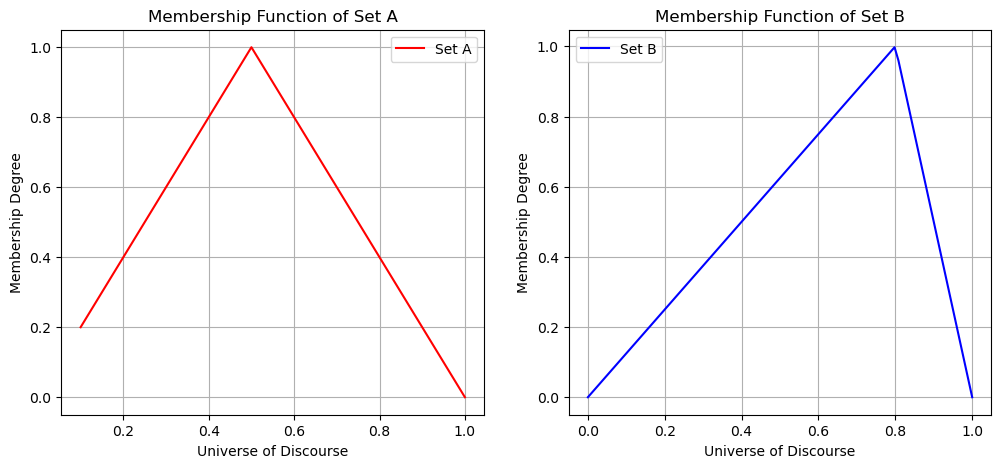
\includegraphics[width=1\textwidth]{output_II_47.png}
\end{center}

\begin{lstlisting}[language=Python]
  union_x, union_y = fuzzy.fuzzy_or(set_a, m_a, set_b, m_b)
  complement_x = fuzzy.fuzzy_not(union_y)
  
  plt.subplots(1, 2, figsize=(12, 5))
  plt.subplot(1, 2, 1)
  plt.plot(union_x, union_y, 'r', label='Union of A and B')
  plt.title('Membership Function of Union of A and B')
  plt.xlabel('Universe of Discourse')
  plt.ylabel('Membership Degree')
  plt.legend()
  plt.grid()
  plt.subplot(1, 2, 2)
  plt.plot(union_x, complement_x, 'b', label='Complement of Union')
  plt.title('Complement of Union of Membership functions A and B')
  plt.xlabel('Universe of Discourse')
  plt.ylabel('Membership Degree')
  plt.legend()
  plt.grid()
\end{lstlisting}

\begin{center}
  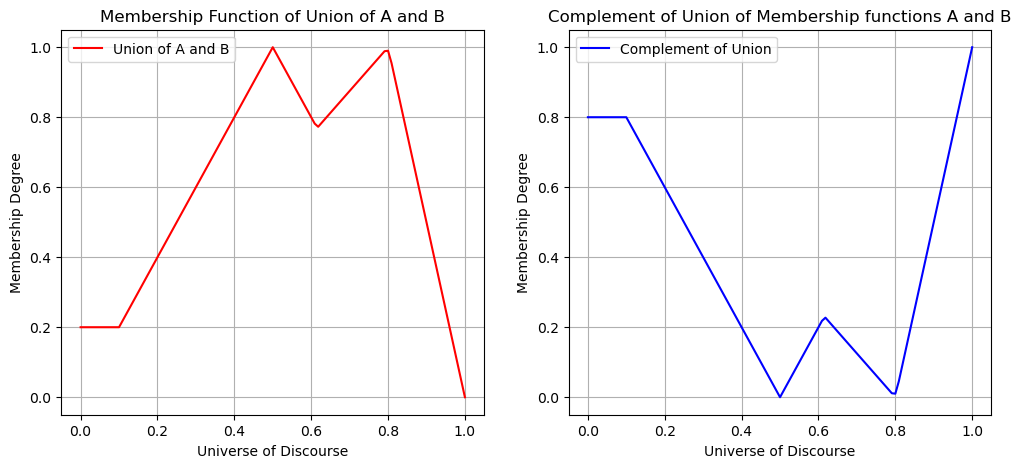
\includegraphics[width=1\textwidth]{output_II_48.png}
\end{center}

\begin{lstlisting}[language=Python]
complement_x = fuzzy.fuzzy_not(m_a)
complement_y = fuzzy.fuzzy_not(m_b)

union_x, union_y = fuzzy.fuzzy_and(set_a, complement_x, set_b, complement_y)

plt.subplots(1, 3, figsize=(18, 5))
plt.subplot(1, 3, 1)
plt.plot(set_a, complement_x, 'r', label='Complement of A')
plt.title('Membership Function of Complement of A')
plt.xlabel('Universe of Discourse')
plt.ylabel('Membership Degree')
plt.legend()
plt.grid()

plt.subplot(1, 3, 2)
plt.plot(set_b, complement_y, 'b', label='Complement of B')
plt.title('Membership Function of Complement of B')
plt.xlabel('Universe of Discourse')
plt.ylabel('Membership Degree')
plt.legend()
plt.grid()

plt.subplot(1, 3, 3)
plt.plot(union_x, union_y, 'g', label='Intersect of Complements of A and B')
plt.title('Intersect of Membership functions of Complements of A and B')
plt.xlabel('Universe of Discourse')
plt.ylabel('Membership Degree')
plt.legend()
plt.grid()
plt.show()
\end{lstlisting}

\begin{center}
  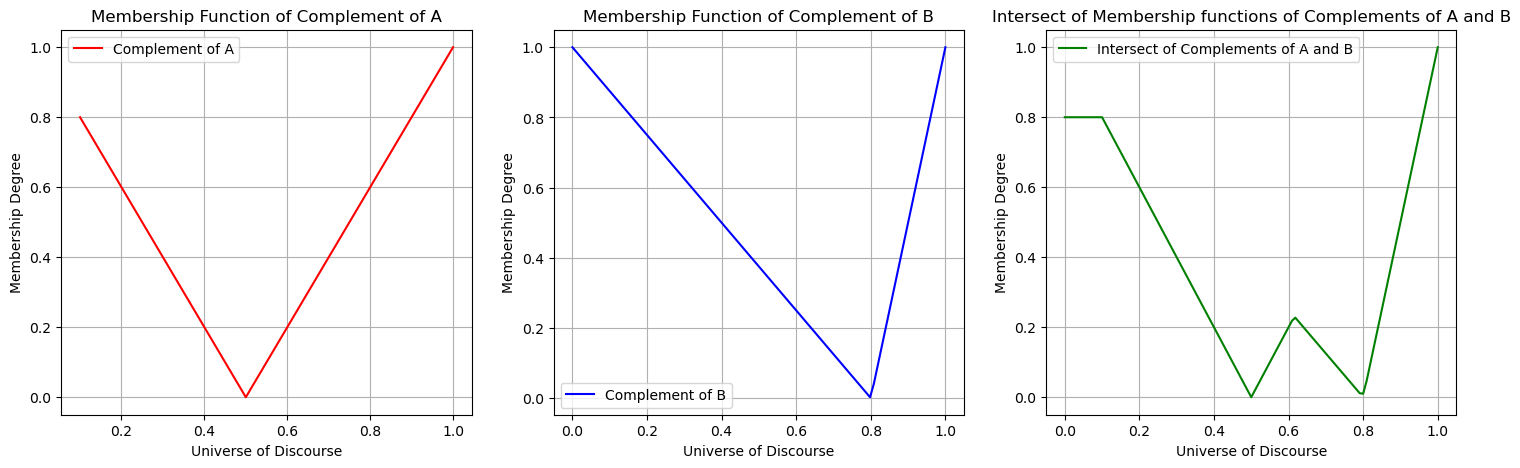
\includegraphics[width=1\textwidth]{output_II_49.png}
\end{center}

\begin{equation*}
\text{De Morgan's second law states that:}
(A \cap B)' = A' \cup B'
\end{equation*}

\begin{lstlisting}[language=Python]
  plt.subplots(1, 2, figsize=(12, 5))
  plt.subplot(1, 2, 1)
  plt.plot(set_a, m_a, 'r', label='Set A')
  plt.title('Membership Function of Set A')
  plt.xlabel('Universe of Discourse')
  plt.ylabel('Membership Degree')
  plt.legend()
  plt.grid()
  plt.subplot(1, 2, 2)
  plt.plot(set_b, m_b, 'b', label='Set B')
  plt.title('Membership Function of Set B')
  plt.xlabel('Universe of Discourse')
  plt.ylabel('Membership Degree')
  plt.legend()
  plt.grid()
\end{lstlisting}

\begin{center}
  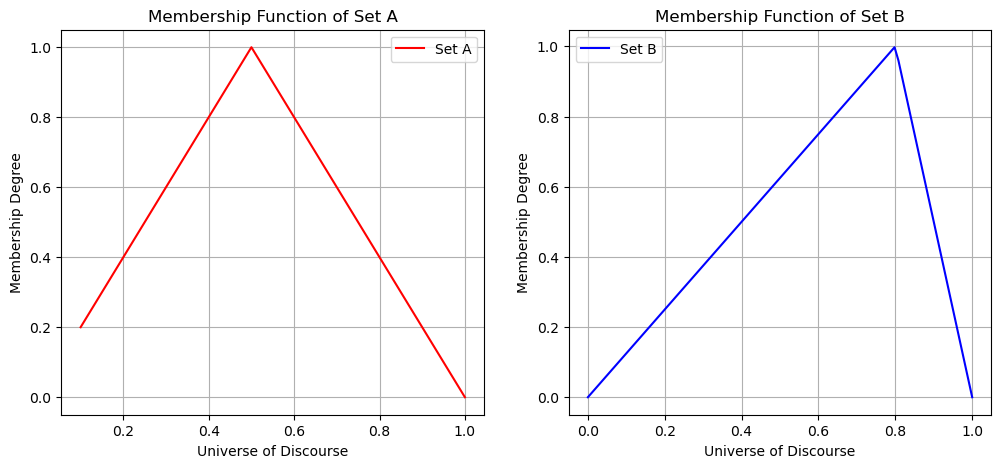
\includegraphics[width=1\textwidth]{output_II_50.png}
\end{center}

\begin{lstlisting}[language=Python]
  intersection_x, intersection_y = fuzzy.fuzzy_and(set_a, m_a, set_b, m_b)
  complement_x = fuzzy.fuzzy_not(intersection_y)
  
  plt.subplots(1, 2, figsize=(12, 5))
  plt.subplot(1, 2, 1)
  plt.plot(intersection_x, intersection_y, 'r', label='Intersection of A and B')
  plt.title('Membership Function of Intersection of A and B')
  plt.xlabel('Universe of Discourse')
  plt.ylabel('Membership Degree')
  plt.legend()
  plt.grid()
  plt.subplot(1, 2, 2)
  plt.plot(union_x, complement_x, 'b', label='Complement of Intersection')
  plt.title('Complement of Intersection of Membership functions A and B')
  plt.xlabel('Universe of Discourse')
  plt.ylabel('Membership Degree')
  plt.legend()
  plt.grid()
\end{lstlisting}

\begin{center}
  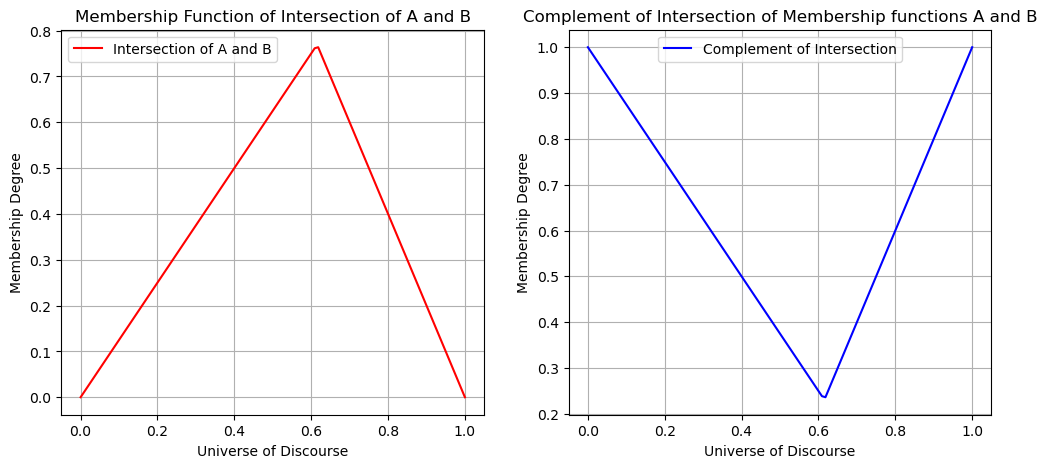
\includegraphics[width=1\textwidth]{output_II_51.png}
\end{center}

\begin{lstlisting}[language=Python]
complement_x = fuzzy.fuzzy_not(m_a)
complement_y = fuzzy.fuzzy_not(m_b)
union_x, union_y = fuzzy.fuzzy_or(set_a, complement_x, set_b, complement_y)
plt.subplots(1, 3, figsize=(18, 5))
plt.subplot(1, 3, 1)
plt.plot(set_a, complement_x, 'r', label='Complement of A')
plt.title('Membership Function of Complement of A')
plt.xlabel('Universe of Discourse')
plt.ylabel('Membership Degree')
plt.legend()
plt.grid()
plt.subplot(1, 3, 2)
plt.plot(set_b, complement_y, 'b', label='Complement of B')
plt.title('Membership Function of Complement of B')
plt.xlabel('Universe of Discourse')
plt.ylabel('Membership Degree')
plt.legend()
plt.grid()
plt.subplot(1, 3, 3)
plt.plot(union_x, union_y, 'g', label='Union of Complements of A and B')
plt.title('Union of Membership functions of Complements of A and B')
plt.xlabel('Universe of Discourse')
plt.ylabel('Membership Degree')
plt.legend()
plt.grid()
plt.show()
\end{lstlisting}

\begin{center}
  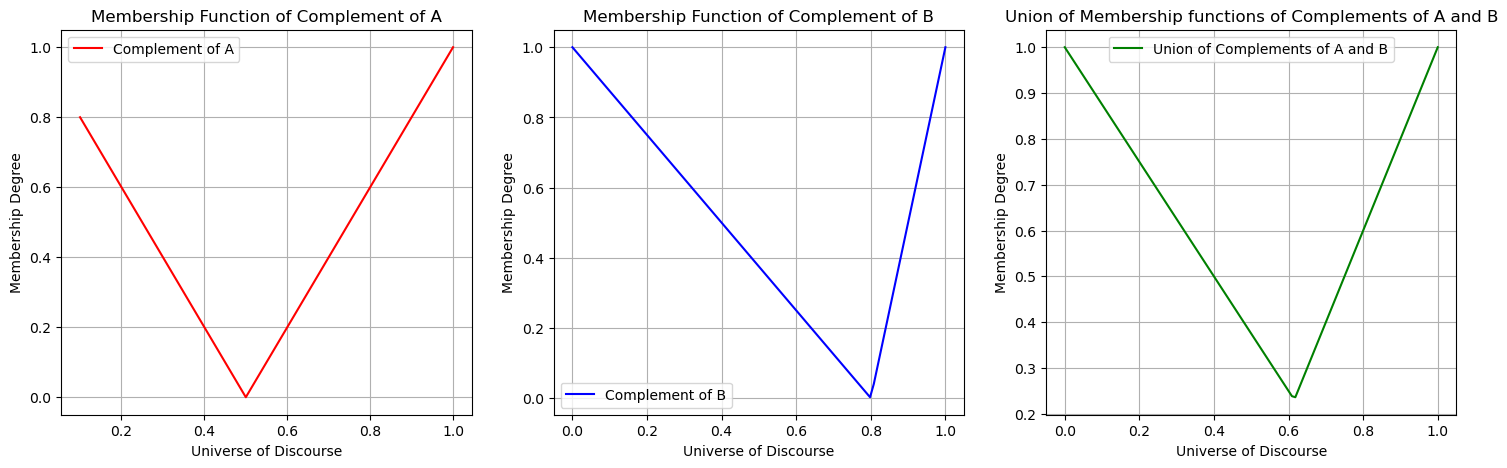
\includegraphics[width=1\textwidth]{output_II_52.png}
\end{center}




\vspace{1em}
\textbf{AI-Generated}

\begin{lstlisting}[language=Python]
import numpy as np
import matplotlib.pyplot as plt

# Define the universe of discourse
x = np.linspace(0, 10, 100)

# Define two fuzzy sets A and B (membership functions)
A = np.maximum(0, 1 - abs(x - 3)/2)  # Triangle centered at 3
B = np.maximum(0, 1 - abs(x - 7)/2)  # Triangle centered at 7

# Fuzzy set operations
union = np.maximum(A, B)
intersection = np.minimum(A, B)
complement_A = 1 - A
complement_B = 1 - B

# De Morgan's Laws
de\_morgan\_1 = 1 - union
de\_morgan\_1\_rhs = np.minimum(complement\_A, complement\_B)

de\_morgan\_2 = 1 - intersection         
de\_morgan\_2\_rhs = np.maximum(complement\_A, complement\_B)

# --- Visualization ---

fig, axs = plt.subplots(3, 2, figsize=(12, 10))
fig.suptitle("Fuzzy Set Operations and De Morgan's Laws", fontsize=16)

# Plot original sets
axs[0, 0].plot(x, A, label='A', color='blue')
axs[0, 0].plot(x, B, label='B', color='red')
axs[0, 0].set_title("Original Fuzzy Sets")
axs[0, 0].legend()
axs[0, 0].grid()

# Union and Intersection
axs[0, 1].plot(x, union, label='A union B', color='purple')
axs[0, 1].plot(x, intersection, label='A intersection B', color='green')
axs[0, 1].set_title("Union and Intersection")
axs[0, 1].legend()
axs[0, 1].grid()

# Complements
axs[1, 0].plot(x, complement_A, label="A'", color='blue', linestyle='--')
axs[1, 0].plot(x, complement_B, label="B'", color='red', linestyle='--')
axs[1, 0].set_title("Complements of A and B")
axs[1, 0].legend()
axs[1, 0].grid()

# De Morgan's Law 1
axs[1, 1].plot(x, de_morgan_1, label="(A union B)'", color='orange')
axs[1, 1].plot(x, de_morgan_1_rhs, label="A' intersection B'", color='green', linestyle='--')
axs[1, 1].set_title("De Morgan's Law 1")
axs[1, 1].legend()
axs[1, 1].grid()

# De Morgan's Law 2
axs[2, 0].plot(x, de_morgan_2, label="(A intersection B)'", color='orange')
axs[2, 0].plot(x, de_morgan_2_rhs, label="A' union B'", color='purple', linestyle='--')
axs[2, 0].set_title("De Morgan's Law 2")
axs[2, 0].legend()
axs[2, 0].grid()

# Hide unused subplot
axs[2, 1].axis('off')

plt.tight_layout(rect=[0, 0, 1, 0.96])
plt.show()
\end{lstlisting}

\vspace{1em}

\textbf{Comments on comparisons}

\begin{itemize}
    \item The AI-generated code uses NumPy and Matplotlib to define and visualize fuzzy sets, while my code uses the skfuzzy library for fuzzy operations.
    \item The AI code visualizes the fuzzy sets and their operations in a single figure with multiple subplots, while my code visualizes each operation in separate figures.
\end{itemize}
\vspace{1em}

\textbf{Results}

\begin{center}
  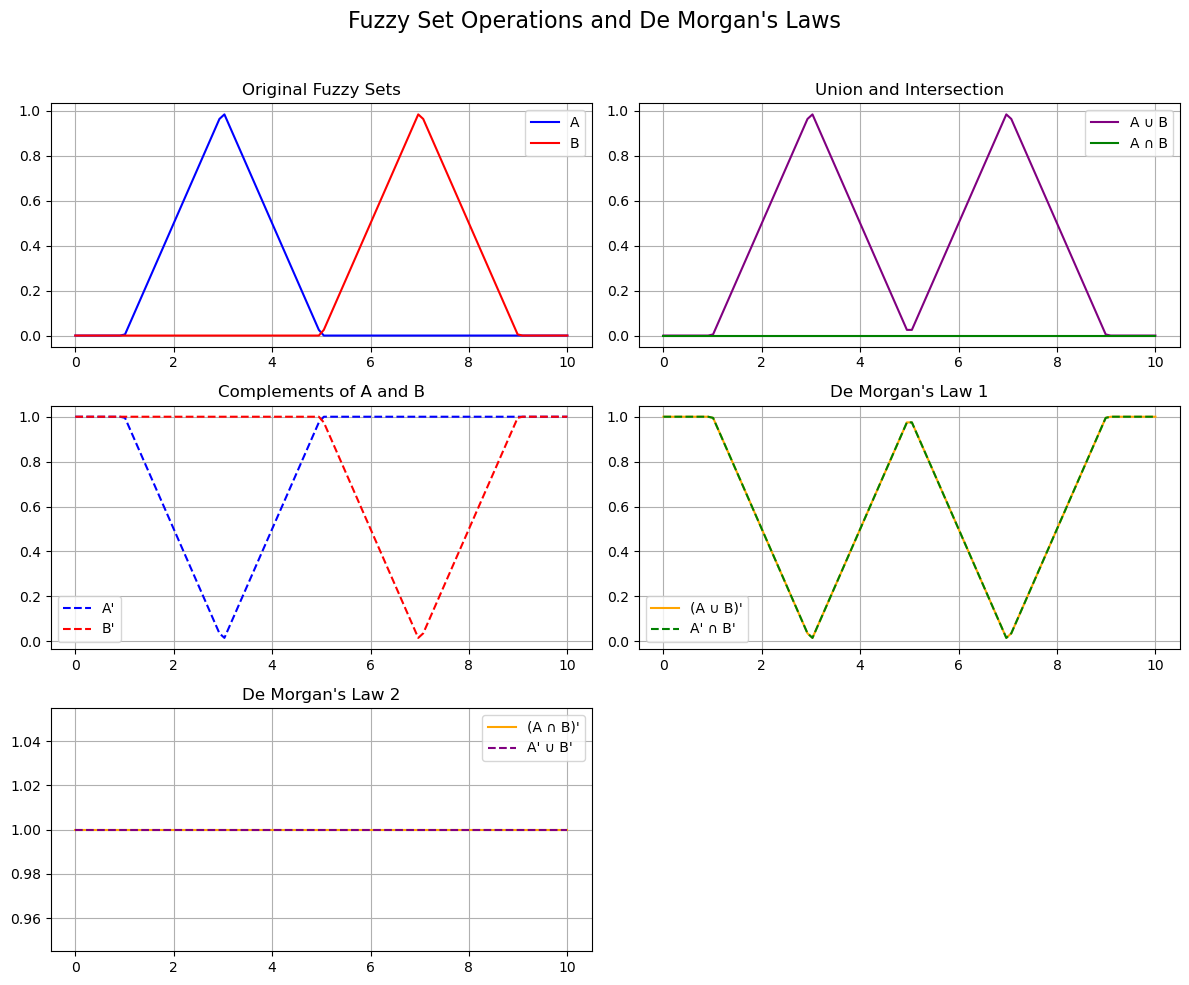
\includegraphics[width=1\textwidth]{output_II_53.png}
\end{center}


\textbf{Verified By}



\end{document}